\documentclass{article}

% if you need to pass options to natbib, use, e.g.:
%     \PassOptionsToPackage{numbers, compress}{natbib}
% before loading neurips_2018

% ready for submission
% \usepackage{neurips_2018}

% to compile a preprint version, e.g., for submission to arXiv, add add the
% [preprint] option:
%     \usepackage[preprint]{neurips_2018}

% to compile a camera-ready version, add the [final] option, e.g.:
     \usepackage[final]{nips_2018}

% to avoid loading the natbib package, add option nonatbib:
%     \usepackage[nonatbib]{neurips_2018}

% Packages to include
\usepackage{helvet}
\usepackage{tikz}
\usepackage{tikz-3dplot}
\usetikzlibrary{backgrounds,3d,shadings,shapes.misc,decorations.pathmorphing,shapes,calc}
%\usepackage{cite}
\usepackage{amssymb,amsmath}
\usepackage{booktabs} % for much better looking tables
\usepackage{mathtools}
%\usepackage{bbding}
\usepackage{graphicx} % support the \includegraphics command and options
\usepackage{subfig}
\usepackage{array} % for better arrays \left(eg matrices\right) in maths
\usepackage{paralist} % very flexible & customisable lists \left(eg. enumerate/itemize, etc.\right)
\usepackage{verbatim} % adds environment for commenting out blocks of text & for better verbatim
\usepackage[labelfont=bf,labelsep=space]{caption} % might need to comment this out in case of conflicts
\usepackage{sectsty} % might need to comment this out in case of conflicts
\usepackage{dblfloatfix} % might need to comment this out in case of conflicts
\usepackage[space]{grffile} % might need to comment this out in case of conflicts
\usepackage{url} % might need to comment this out in case of conflicts
\usepackage[toc]{appendix} % might need to comment this out in case of conflicts
\usepackage[titles,subfigure]{tocloft} % Alter the style of the Table of Contents. Might need to comment this out in case of conflicts
%\usepackage{geometry} % to change the page dimensions
%\geometry{letterpaper}
\usepackage[breakable, theorems, skins]{tcolorbox}
\usepackage{algorithm} % algorithms
\usepackage[noend]{algpseudocode} % algorithms
%\usepackage{hyperref}
\usepackage{pgfplots}
\usepackage{cancel}
\usepackage{bm}
\newcommand{\bs}[1]{\bm{\mathrm{#1}}}

% ---- Definitions ----

% Template for algorithms, source: https://tex.stackexchange.com/questions/163768/write-pseudo-code-in-latex

%\begin{algorithm}
%	\caption{Meta-pruning for weights} \label{alg1}
%	\begin{algorithmic}[1]
%		\Procedure{MyProcedure}{}
%		\State $\textit{stringlen} \gets \text{length of }\textit{string}$
%		\State $i \gets \textit{patlen}$
%		\BState \emph{top}:
%		\If {$i > \textit{stringlen}$} \Return false
%		\EndIf
%		\State $j \gets \textit{patlen}$
%		\BState \emph{loop}:
%		\If {$\textit{string}(i) = \textit{path}(j)$}
%		\State $j \gets j-1$.
%		\State $i \gets i-1$.
%		\State \textbf{goto} \emph{loop}.
%		\State \textbf{close};
%		\EndIf
%		\State $i \gets i+\max(\textit{delta}_1(\textit{string}(i)),\textit{delta}_2(j))$.
%		\State \textbf{goto} \emph{top}.
%		\EndProcedure
%	\end{algorithmic}
%\end{algorithm}



% Coloured boxes for highlighting text, e.g. for summaries, theorems, etc.
\DeclareRobustCommand{\colourbox}[2][gray!20]{%
	\begin{tcolorbox}[   %% Adjust the following parameters at will.
		breakable,
		left=0pt,
		right=0pt,
		top=0pt,
		bottom=0pt,
		colback=#1,
		colframe=#1,
		width=\dimexpr\textwidth\relax, 
		enlarge left by=0mm,
		boxsep=5pt,
		arc=0pt,outer arc=0pt,
		]
		#2
	\end{tcolorbox}
}


% ---- My definitions ----
%\DeclareMathOperator{\pv}{pv}
%\DeclareMathOperator{\sign}{sign}
%\DeclareMathOperator{\ber}{ber}
%\DeclareMathOperator{\bei}{bei}
%\newcommand{\vect}[1]{\mathbf{#1}}
%\newcommand{\nhat}{\mathbf{\hat{n}}}
\newcommand{\vect}[1]{\vec{#1}}
\newcommand{\nhat}{{\hat{n}}}
\newcommand{\nvec}{{\hat{n}}}
\newcommand{\ver}[1]{\hat{#1}}
%\newcommand{\matr}[1]{\mathbf{#1}}
\newcommand{\matr}[1]{\bs{#1}}
\newcommand{\abs}[1]{\left \lvert #1 \right\rvert }
\newcommand{\norm}[1]{ \left \lVert #1 \right \rVert} 
%\newcommand{\pvint}{\pv\!\!\int}
\newcommand{\pvint}{\dashint}
\newcommand{\intR}{\int_{-\infty}^{+\infty}}
\newcommand{\pvintR}{\pvint_{-\infty}^{+\infty}}
\newcommand{\laplace}[1]{\mathscr{L}\{#1\}}
\newcommand{\ilaplace}[1]{\mathscr{L}^{-1}\{#1\}}
\newcommand{\blaplace}[1]{\mathscr{L}_b\{#1\}}
\newcommand{\fourier}[1]{\mathscr{F}\{#1\}}
\newcommand{\ifourier}[1]{\mathscr{F}^{-1}\{#1\}}
\renewcommand{\Re}[1]{\mathbb{R}\mathrm{e}\left \{#1\right\} }
\renewcommand{\Im}[1]{\mathbb{I}\mathrm{m}\left \{#1\right\} }
\newcommand{\Real}{\mathbb{R}}
\newcommand{\Complex}{\mathbb{C}}
% Sets
\newcommand{\complem}[1]{#1^{\rm C}}
\newcommand{\expon}[1]{\operatorname{e}^{\,#1}}
\newcommand{\ns}{\!\!\!\!}
\newcommand{\pref}[1]{(\ref{#1})}
\newcommand{\junk}[1] {}
\newcommand{\missing}[1]{\vspace*{\parskip}
			\centerline{\framebox{\begin{minipage}{0.9\columnwidth}{\large\bf\noindent #1}
				\end{minipage}}}
			\vspace*{\parskip}}


% Principal value integral sign
\def\Xint#1{\mathchoice
{\XXint\displaystyle\textstyle{#1}}%
{\XXint\textstyle\scriptstyle{#1}}%
{\XXint\scriptstyle\scriptscriptstyle{#1}}%
{\XXint\scriptscriptstyle\scriptscriptstyle{#1}}%
\!\int}
\def\XXint#1#2#3{{\setbox0=\hbox{$#1{#2#3}{\int}$}
\vcenter{\hbox{$#2#3$}}\kern-.5\wd0}}
\def\ddashint{\Xint=}
\def\dashint{\Xint-}

\newcommand*\widebar[1]{%
  \hbox{%
    \vbox{%
      \hrule height 0.5pt % The actual bar
      \kern0.3ex%         % Distance between bar and symbol
      \hbox{%
        \kern-0.05em%      % Shortening on the left side
        \ensuremath{#1}%
        \kern-0.05em%      % Shortening on the right side
      }%
    }%
  }%
} 


\renewcommand{\epsilon}{\varepsilon}

\newcommand{\dbd}[2]{\ensuremath{\dfrac{d#1}{d#2}}}
\newcommand{\ddt}[1]{\ensuremath{\dfrac{d#1}{dt}}}
\newcommand{\ddx}[1]{\ensuremath{\dfrac{d#1}{dx}}}
\newcommand{\ddy}[1]{\ensuremath{\dfrac{d#1}{dy}}}
\newcommand{\ddz}[1]{\ensuremath{\dfrac{d#1}{dz}}}

\newcommand{\pardt}[1]{\ensuremath{\dfrac{\partial#1}{\partial t}}}
\newcommand{\pardx}[1]{\ensuremath{\dfrac{\partial#1}{\partial x}}}
\newcommand{\pardy}[1]{\ensuremath{\dfrac{\partial#1}{\partial y}}}
\newcommand{\pardz}[1]{\ensuremath{\dfrac{\partial#1}{\partial z}}}

\newcommand{\pardtsq}[1]{\ensuremath{\dfrac{\partial^2#1}{\partial t^2}}}
\newcommand{\pardxsq}[1]{\ensuremath{\dfrac{\partial^2#1}{\partial x^2}}}
\newcommand{\pardysq}[1]{\ensuremath{\dfrac{\partial^2#1}{\partial y^2}}}
\newcommand{\pardzsq}[1]{\ensuremath{\dfrac{\partial^2#1}{\partial z^2}}}

\newcommand{\curl}[1]{\ensuremath{\nabla\times\bs{#1}}}
\newcommand{\tensor}[1]{\ensuremath{\bar{\bar{#1}}}}

\newcommand{\figref}[1]{Figure~\ref{#1}}
\newcommand{\algoref}[1]{Algorithm~\ref{#1}}
\newcommand{\secref}[1]{Section~\ref{#1}}
\newcommand{\tabref}[1]{Table~\ref{#1}}

\newcommand{\opL}{\mathcal{L}} % L operator
\newcommand{\opK}{\mathcal{K}} % K operator

% Theorems, laws, definitions environments
\newtheorem{defn}{Definition}
\newtheorem{thm}{Theorem}
\newtheorem{exm}{Example}
\newtheorem{rmk}{Remark}


\usepackage{listings}
\usepackage{color}

\definecolor{mygreen}{RGB}{28,172,0} % color values Red, Green, Blue
\definecolor{mylilas}{RGB}{170,55,241}

\lstset{language=Matlab,%
	%basicstyle=\color{red},
	basicstyle=\ttfamily,
	breaklines=true,%
	morekeywords={matlab2tikz},
	%keywordstyle=\color{blue},%
	morekeywords=[2]{1}, keywordstyle=[2]{\color{black}},
	identifierstyle=\color{black},%
	stringstyle=\color{mylilas},
	commentstyle=\color{mygreen},%
	showstringspaces=false,%without this there will be a symbol in the places where there is a space
	numbers=left,%
	numberstyle={\tiny \color{black}},% size of the numbers
	numbersep=9pt, % this defines how far the numbers are from the text
	emph=[1]{for,end,break},emphstyle=[1]\color{blue}, %some words to emphasise
	%emph=[2]{word1,word2}, emphstyle=[2]{style},    
}



% For algorithms
\makeatletter
\def\BState{\State\hskip-\ALG@thistlm}
\makeatother

\usepackage[utf8]{inputenc} % allow utf-8 input
\usepackage[T1]{fontenc}    % use 8-bit T1 fonts
%\usepackage{hyperref}       % hyperlinks
\usepackage{url}            % simple URL typesetting
\usepackage{booktabs}       % professional-quality tables
\usepackage{amsfonts}       % blackboard math symbols
\usepackage{nicefrac}       % compact symbols for 1/2, etc.
\usepackage{microtype}      % microtypography

\title{Iterative Network Pruning for Improved Performance and Generalization}

% The \author macro works with any number of authors. There are two commands
% used to separate the names and addresses of multiple authors: \And and \AND.
%
% Using \And between authors leaves it to LaTeX to determine where to break the
% lines. Using \AND forces a line break at that point. So, if LaTeX puts 3 of 4
% authors names on the first line, and the last on the second line, try using
% \AND instead of \And before the third author name.

\author{%
  Adriana~Salcedo\\
  Department of Medical Biophysics\\
  University of Toronto\\
  Toronto, ON M5S 1A1\\
  \texttt{a.salcedo@mail.utoronto.ca} \\
  % examples of more authors
   \And
   Shashwat~Sharma\\
   Edward S.~Rogers~Sr. Department of Electrical \& Computer Engineering \\
   University of Toronto\\
   Toronto, ON M5S 1A1\\
   \texttt{shash.sharma@mail.utoronto.ca} \\
  % \AND
  % Coauthor \\
  % Affiliation \\
  % Address \\
  % \texttt{email} \\
  % \And
  % Coauthor \\
  % Affiliation \\
  % Address \\
  % \texttt{email} \\
  % \And
  % Coauthor \\
  % Affiliation \\
  % Address \\
  % \texttt{email} \\
}

\begin{document}
% \nipsfinalcopy is no longer used

\maketitle

\begin{abstract}
  Neural networks are commonly designed to have extremely large numbers of trainable parameters to obtain accurate models for complex problems. Yet the actual number of parameters needed to describe the model may be significantly smaller than the initial choice. Pruning is a commonly used strategy to reduce the size of an existing network by removing parameters that are relatively less important. This reduces memory and time requirements when deploying the model. Pruning has also been shown to improve the ability of a model to generalize. In this work, we study two classes of simple methods to prune an existing model, and extend those methods in the context of generalization, by iteratively training on multiple related datasets, while pruning the model. We show that pruning does indeed yield smaller and sparser models without serious detriment to model accuracy, and that pruning does, to some extent, have a beneficial impact on the model's ability to generalize.
\end{abstract}

\section{Introduction}

Modern neural networks tend to be immensely large with several millions of connections and weights. The memory and energy requirements for deploying such networks is significant, and constantly growing with the complexity of state-of-the-art networks. Although having a large number of trainable parameters is beneficial to network accuracy, it was shown by \citet{NIPS_learning_weights_pruning}, \citet{OBD} and \citet{OBS} that the impact of some parameters is negligible in comparison with others. Successful identification and removal (``pruning'') of such parameters would lead to smaller and faster networks, which in turn would significantly reduce the computational cost at test time. The goal of most pruning algorithms is to achieve computational advantages without an appreciable impact on accuracy. The importance and relevance of network pruning was recently highlighted via MorphNet, proposed by \citet{morphnet} at Google to optimize existing networks through pruning.

It was argued by \citet{prune_transfer_learning} that pruning can also be applied in the context of transfer learning, for generalization of a trained network to related datasets. Improved ability of networks to generalize as a result of pruning was also achieved by \citet{prune_for_architecture}. However, these approaches target networks that have been trained on a single dataset. In contrast, the concept of learning the hyperparameters of a network by using multiple datasets, known as ``meta-learning", has also been proposed by \citet{maml}. To the best of our knowledge, the meta-learning concept has not been applied in the context of network pruning.

The above points motivate the main idea proposed in this work: designing pruning methodologies that specifically target improved generalization of a given network, by leveraging multiple datasets during training. The goal is to optimize existing networks not only to be faster and smaller, but also to improve their ability to generalize. We first implement and study some simple and commonly-used pruning strategies and analyze their impact on network size, speed and accuracy. We then discuss and implement a simple meta-learning algorithm and study its performance. Finally, we combine the pruning strategies with the meta-learning algorithm to introduce a proof-of-concept ``meta-pruning'' methodology. The general outline and structure of this paper are summarized in \figref{summaryFig}.

\begin{figure}[t]
	\centering
	
	% Define block styles
	\tikzstyle{decision} = [diamond, draw, fill=blue!20, 
	text width=4.5em, text badly centered, node distance=3cm, inner sep=0pt]
	\tikzstyle{block} = [rectangle, draw, fill=blue!10, 
	text width=5em, text centered, rounded corners, minimum height=2em]
	\tikzstyle{line} = [draw, -latex', thick]
	\tikzstyle{cloud} = [draw, rectangle, rounded corners, fill=red!20, node distance=2cm,
	minimum height=4em, text width=8em]
	\tikzstyle{heading} = [draw=none, ellipse, fill=none,
	minimum height=2em]
	
	\begin{tikzpicture}[node distance = 2cm, auto, >=latex]
	% Place nodes
	\node [heading] (survey) {\textbf{Survey on Simple Pruning Methods}};
	\node [block, below left of=survey, node distance=2cm] (surveyClass) {Classifier};
	\node [block, right of=surveyClass, node distance=3cm] (surveyFeature) {Features};
%	
	\node [cloud, below left of=surveyClass, node distance=3cm] (surveyClass1) {Masking based on a threshold};
	\node [cloud, below of=surveyClass1, node distance=2cm] (surveyClass2) {Learned masking based on L0 norm};
%	
	\node [cloud, below right of=surveyFeature, node distance=3cm] (surveyFeature1) {Pruning filters based on accumulated activation or weight norms};
	\node [cloud, below of=surveyFeature1, node distance=2cm] (surveyFeature2) {Learned masking based on L0 norm};
%
	\node [heading, below of=survey, node distance=7.0cm] (multidat) {\textbf{Pruning with Multiple Datasets for Generalization}};
	\node [block, below left of=multidat, node distance=2cm] (multidatClass) {Classifier};
	\node [block, right of=multidatClass, node distance=3cm] (multidatFeature) {Features};
	%	
	\node [cloud, below left of=multidatClass, node distance=3cm] (multidatClass1) {Intersection pruning with threshold-based masking};
	\node [cloud, below of=multidatClass1, node distance=2cm] (multidatClass2) {Meta-pruning based on REPTILE with learned masking};
	%	
	\node [cloud, below right of=multidatFeature, node distance=3cm] (multidatFeature1) {Intersection pruning with accumulated activation- or weight-norm based filter pruning};
%	
%	% Draw edges
	\path [line] (survey) -- (surveyClass);
	\path [line] (survey) -- (surveyFeature);
	\path [line] (surveyClass) |- (surveyClass1);
	\path [line] (surveyClass) |- (surveyClass2);
	\path [line] (surveyFeature) |- (surveyFeature1);
	\path [line] (surveyFeature) |- (surveyFeature2);
%	
	\path [line] (multidat) -- (multidatClass);
	\path [line] (multidat) -- (multidatFeature);
	\path [line] (multidatClass) |- (multidatClass1);
	\path [line] (multidatClass) |- (multidatClass2);
	\path [line] (multidatFeature) |- (multidatFeature1);
%	\path [line] (multidatFeature) |- (multidatFeature2);
	\end{tikzpicture}
	\vspace{4mm}
	\caption{Outline of this paper.}
	\label{summaryFig}
\end{figure}

\section{Formal Description}

In this section, we describe the two main phases of this work. First, we present a survey on simple pruning algorithms that have been presented in literature, to study their effect on network performance. Second, we propose combinations of pruning with the concept of meta-learning to leverage multiple datasets, to improve model generalizability while pruning.

\subsection{A Survey on Simple Pruning Algorithms}

Three simple approaches to pruning are reviewed below. The first two focus on pruning the classifier layers of the network, while the third involves pruning convolution layers.

\subsubsection{Masking of Classifier Layers Based on a Threshold} \label{MaskClass}

We pruned weights of the linear and / or convolution layers based on their absolute value, as proposed by \citet{NIPS_learning_weights_pruning}. To focus on the effects of pruning, we did not add an L2 penalty or drop-out layers, and instead only added a mask term in the forward pass of the linear and/or convolution layers. Every five epochs, we eliminated the weights with absolute values in the $p$ lowest proportion. The mask itself was not optimized, but the threshold was adjusted every five epochs. Results are shown in \figref{f1}.

\begin{figure}[!t]
	\centering
	\subfloat[][]
	{
		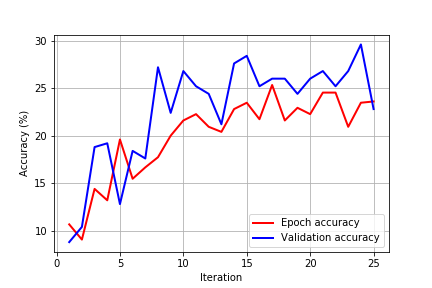
\includegraphics[width=6cm]{./Figures/Fig1/A_baseline_10_accuracy.png}
	}
	\subfloat[][]
	{
		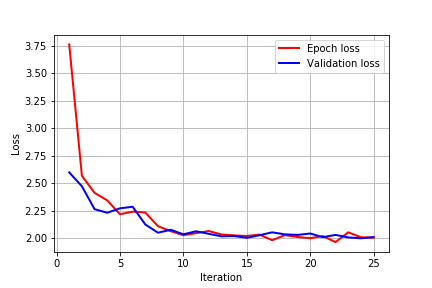
\includegraphics[width=6cm]{./Figures/Fig1/B_baseline_10_loss.png}
	}\\
	\subfloat[][]
	{
		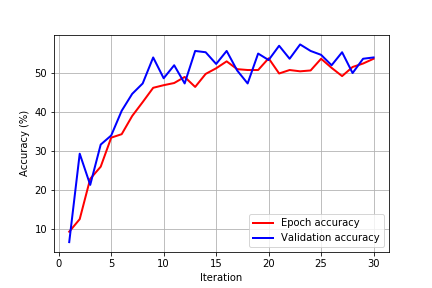
\includegraphics[width=6cm]{./Figures/Fig1/C_baseline_T_accuracy.png}
	}
	\subfloat[][]
	{
		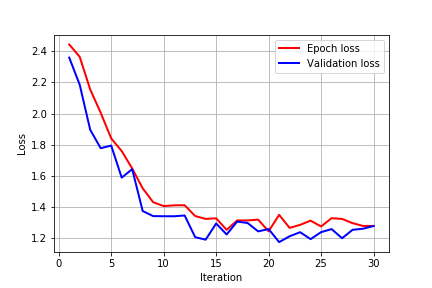
\includegraphics[width=6cm]{./Figures/Fig1/D_baseline_T_loss.png}
	}\\
	\subfloat[][]
	{
		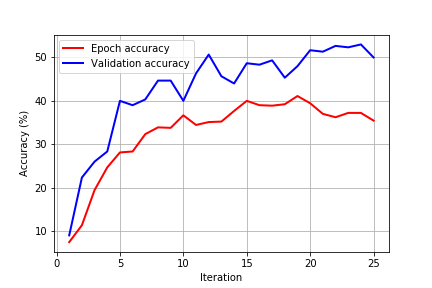
\includegraphics[width=6cm]{./Figures/Fig1/E_ct0_T_accuracy.png}
	}
	\subfloat[][]
	{
		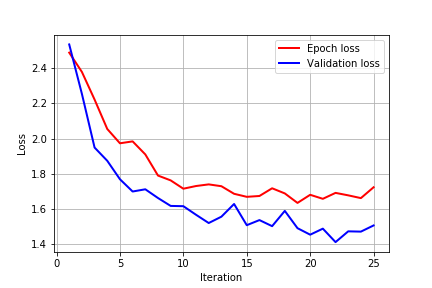
\includegraphics[width=6cm]{./Figures/Fig1/F_ct0_T_loss.png}
	}\\
	\subfloat[][]
	{
		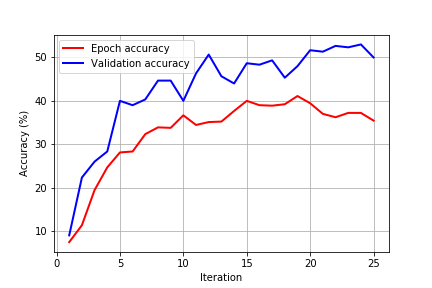
\includegraphics[width=6cm]{./Figures/Fig1/G_ct0_T_accuracy1.png}
	}
	\subfloat[][]
	{
		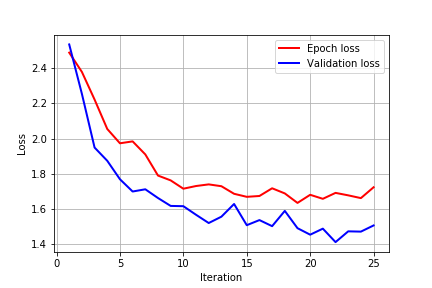
\includegraphics[width=6cm]{./Figures/Fig1/H_ct0_T_loss1.png}
	}
	\caption{A. Baseline accuracy on CIFAR-10. B. Baseline loss on CIFAR-10.  C. Fine-tuning accuracy of VGG-16 on fashion MNIST after training on CIFAR-10. D. Fine-tuning loss of VGG-16 on fashion MNIST after training on CIFAR 10. E. Threshold pruning accuracy on CIFAR-10. F. Threshold pruning loss on CIFAR-10.  G. Fine-tuning accuracy of VGG16 on fashion MNIST after training on CIFAR-10 with threshold-pruning. H. Fine-tuning loss of VGG-16 on fashion MNIST after training on CIFAR-10 with threshold pruning.}
	\label{f1}
\end{figure}

\subsubsection{Learned Masking of Classifier Layers} \label{MaskClassL0}

\citet{L0norm} recently proposed a method to learn a pruning mask throughout training by applying a learnable L0 penalty. The L0 is a nearly binary mask based on the hard-concrete distribution that is applied to the inputs for each weight. Although the L0 mask is nearly binary, because of its probabilistic formulation it is possible to differentiate through it, unlike with a binary mask. The number of non-zero terms in the mask is then added to the loss, encouraging sparsity as training proceeds. We implemented the L0 penalty in both the classifier and convolution layers, but found that the performance on convolution layers was detrimental to the network. Thus for the L0-based pruning, we focus on the classifier layer. Results are shown in \figref{f2}.

\begin{figure}[!t]
	\centering
	\subfloat[][]
	{
		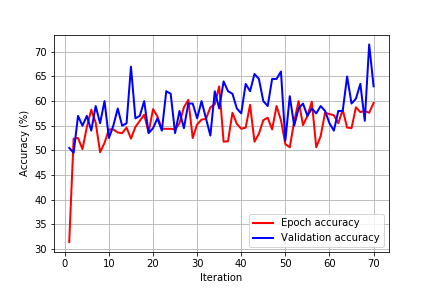
\includegraphics[width=6cm]{./Figures/Fig2/A_ip_cifar_accuracy.png}
	}
	\subfloat[][]
	{
		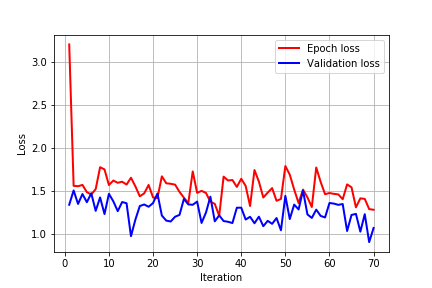
\includegraphics[width=6cm]{./Figures/Fig2/B_ip_cifar_loss.png}
	}\\
	\subfloat[][]
	{
		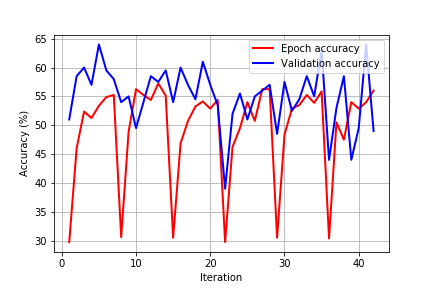
\includegraphics[width=6cm]{./Figures/Fig2/C_ip_cifar_mask_accuracy.png}
	}
	\subfloat[][]
	{
		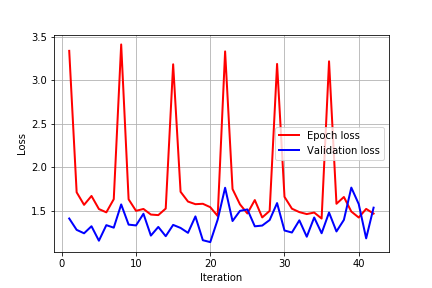
\includegraphics[width=6cm]{./Figures/Fig2/D_ip_cifar_mask_loss.png}
	}\\
	\subfloat[][]
	{
		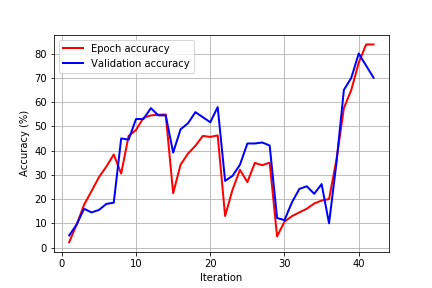
\includegraphics[width=6cm]{./Figures/Fig2/E_ip_multiple_accuracy.png}
	}
	\subfloat[][]
	{
		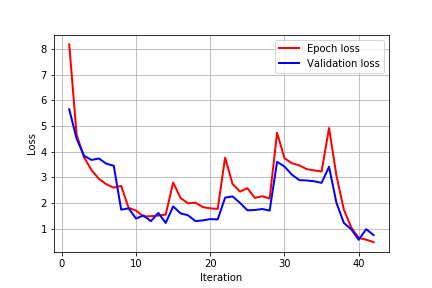
\includegraphics[width=6cm]{./Figures/Fig2/F_ip_multiple_loss.png}
	}
	\caption{A. Iterative pruning accuracy subsampling CIFAR-10. B. Iterative pruning loss subsampling CIFAR-10. C. Iterative pruning accuracy subsampling CIFAR-10 re-initializing weights at each outer-iteration. D. Iterative pruning loss subsampling CIFAR-10 re-initializing weights at each outer-iteration. E. Iterative pruning accuracy subsampling multiple datasets. F. Iterative pruning loss subsampling  multiple datasets}
	\label{f2}
\end{figure}

\subsubsection{Pruning Convolution Filters} \label{PruneFilter}

One method to prune convolutional layers is to reduce the number of output channels in each layer, which involves reducing the size of associated weight matrices. This impacts not only the convolution layer being pruned, but also the number of input channels in the next layer of the network. This approach was proposed by \cite{prune_transfer_learning}, and has since been implemented via open-source code provided by \cite{jacobgilblog}. However, this implementation only allows for pruning a single output channel at a time. We have implemented a version of this technique that allows pruning out several filters simultaneously, greatly improving the efficiency of aforementioned the code.

Although a relatively sophisticated strategy for picking pruned channels was presented by \cite{prune_transfer_learning}, in our implementation we use two simple metrics to decide which channels are to be pruned: the 2-norm of the layer's activations, and the 2-norm of weights. In each case, pruning occurs after every $N_i$ epochs, until training is complete. The number of output channels to prune, $N_p$, is set via the hyperparameter $p$, which is a percentage of the total available parameters in that network, $N_\mathrm{total}$:
\begin{align}
	N_p = \mathrm{round} \left(\dfrac{p}{100}N_\mathrm{total}\right). \label{eqNp}
\end{align}
In the activation-based approach, the activations of each layer are accumulated over the $N_i$ epochs preceding a single pruning pass via the function \texttt{TrackConv2DNorms}. This is done as follows: at each training iteration, we compute the 2-norm of the activations of each layer, across all of the input data dimensions (function \texttt{ComputeConv2DActNorms}). The output of this is a vector whose size is the number of output channels of a particular layer, and one such vector is constructed for each convolution layer. These vectors represent the strength of the activations of each filter. Optionally, these vectors can be normalized to their maximum values to ensure that every set of $N_i$ epochs is equally represented.

The new activation norm vectors computed at each iteration are added to the previously stored vectors. Every $N_i$ epochs, we look at the accumulated activation vector and extract the indices corresponding to the $N_p$ smallest activations (function \texttt{PruneAllConv2DLayers}). This tells us the $N_p$ filters of each layer which had, on average, the weakest activations over the last $N_i$ epochs. Those filters are then pruned away, and the old model is replaced with the updated, smaller model (function \texttt{PruneConvLayers}). At this stage, the accumulated activation norm vectors are reset to their initial state, ready to start accumulating activations for the next $N_i$ epochs.

When pruning based on weights, the strategy is the same as above, except that rather than accumulating activations, we accumulate the 2-norms of the weight matrices themselves. The 2-norms are computed over the input channel dimension, and over the kernel of each filter (function \texttt{ComputeConv2DWeightNorms}). Again, this yields, for each layer, a vector containing 2-norms corresponding to the weights of each output channel. This can also be optionally normalized to the maximum value in each vector. Every $N_i$ epochs, these accumulated vectors are used to prune away the weakest $N_p$ filters.

The methodology described above is summarized in \algoref{FilterPruneBasic}, \algoref{FilterPruneComps} and \algoref{FilterPruneDrivers}.
The results of both methods in comparison to the baseline (no pruning) are discussed below.

\begin{algorithm}[t]
	\caption{Helper functions for iterative convolution filter pruning - single dataset} \label{FilterPruneBasic}
	\begin{algorithmic}[1]
		\Function{ComputeConv2DWeightNorms}{${\mathrm{model}, \matr{n}_w}$}
			\For {all $i$ in $\textit{convolution layers of }\mathrm{model}$}
				\State $\widetilde{\matr{n}}_{w,i} \gets \textit{2-norm of weights of layer }i\textit{ across dims 1, 2, 3}$
				\State $\widetilde{\matr{n}}_{w,i} \gets \widetilde{\matr{n}}_{w,i} / \max\abs{\widetilde{\matr{n}}_{w,i}} \textit{ (optional)}$
				\State $\matr{n}_{w,i} \gets \textit{append }\widetilde{\matr{n}}_{w,i}$
			\EndFor
			\State \Return $\matr{n}_{w,i}$
		\EndFunction
		\\
	%	
		\Function{ComputeConv2DActNorms}{${\mathrm{model}, \matr{n}_a}$}
			\For {all $i$ in $\textit{convolution layers of }\mathrm{model}$}
				\State $\widetilde{\matr{n}}_{a,i} \gets \textit{2-norm of activations of layer }i\textit{ across dims 0, 2, 3}$
				\State $\widetilde{\matr{n}}_{a,i} \gets \widetilde{\matr{n}}_{a,i} / \max\abs{\widetilde{\matr{n}}_{a,i}} \textit{ (optional)}$
				\State $\matr{n}_{a,i} \gets \textit{append }\widetilde{\matr{n}}_{a,i}$
			\EndFor
			\State \Return $\matr{n}_{a,i}$
		\EndFunction
%
	\end{algorithmic}
\end{algorithm}


\begin{algorithm}[t]
	\caption{Computational functions for iterative convolution filter pruning - single dataset} \label{FilterPruneComps}
	\begin{algorithmic}[1]
		\Function{PruneConvLayers}{${\matr{l}_\mathrm{idx}, \matr{f}_\mathrm{idx}, \mathrm{model}}$}
			\State $\matr{c}_\mathrm{idx} \gets \matr{l}_\mathrm{idx}^\mathrm{th}\textit{ conv layer of } \mathrm{model}$
			\State $\matr{w}_0 \gets \textit{weights of  } \matr{c}_\mathrm{idx}$
			\State $\matr{w}_0 \gets \textit{delete entries corresponding to filters in }\matr{f}_\mathrm{idx}$
			\State $\matr{c}_\mathrm{idx} \gets \textit{copy updated weights }\matr{w}_0$
			\State $\mathrm{model} \gets \textit{updated conv layer }\matr{c}_\mathrm{idx} \textit{ at layer }\matr{l}_\mathrm{idx}$
			\State \Return $\mathrm{model}$
		\EndFunction
		\\
		%		
		\Function{PruneAllConv2DLayers}{${\matr{n}_{a}, \matr{n}_{w}, N_p, \mathrm{model}}$}
		\For {all $i$ in $\textit{convolution layers of }\mathrm{model}$}
			\If {\textit{activation-based pruning}}
				\State $\matr{n}_{i} \gets \matr{n}_{a,i}$
			\ElsIf {\textit{weight-based pruning}}
				\State $\matr{n}_{i} \gets \matr{n}_{w,i}$
			\EndIf
			\State $\matr{f}_\mathrm{idx,i} \gets \textit{indices of bottom $N_p$ elements of }\matr{n}_{i}$
			\State $\mathrm{model} \gets$ \Call{PruneConvLayers}{${i, \matr{f}_\mathrm{idx,i}, \mathrm{model}}$}
		\EndFor
%		
		\State \Return $\mathrm{model}$
		\EndFunction
		%
	\end{algorithmic}
\end{algorithm}

\begin{algorithm}[t]
	\caption{Driver functions for iterative convolution filter pruning - single dataset} \label{FilterPruneDrivers}
	\begin{algorithmic}[1]
			\Function{TrainModel}{$\mathrm{model}, \mathrm{input}, N_i, N_p$}
			\For {all $i$ in $\mathrm{input}$}
				\State $\matr{n}_{a} +\gets$ \Call{ComputeConv2DActNorms}{${\mathrm{model}, \matr{n}_{a}}$}
				\State $\matr{n}_{w} +\gets$ \Call{ComputeConv2DWeightNorms}{${\mathrm{model}, \matr{n}_{w}}$}
				\If {$i \% N_i == 0$}
					\State $\mathrm{model} \gets$ \Call{PruneAllConv2DLayers}{${\matr{n}_{a}, \matr{n}_{w}, N_p, \mathrm{model}}$}
					\State $\matr{n}_{a} \gets \textit{reset}$
					\State $\matr{n}_{w} \gets \textit{reset}$
				\EndIf
			\EndFor
			%		
			\State \Return $\mathrm{model}$
		\EndFunction\\
%		
		\State $\mathrm{model} \gets \textit{VGG16}$
		\State $p \gets 5$
		\State $N_p \gets \textit{value as per \eqref{eqNp}}$
		\State $N_i \gets 7$
		\State $\mathrm{input} \gets \textit{sample 10\% of data from CIFAR-10}$
		\While {$i < 50$}
			\State $\mathrm{model} \gets $ \Call{TrainModel}{$\mathrm{model}, \mathrm{input}, N_i, N_p$}
		\EndWhile
		%
	\end{algorithmic}
\end{algorithm}


\begin{algorithm}[t]
	\caption{Driver function for meta convolution filter pruning - multiple datasets} \label{FilterPruneDriverMeta}
	\begin{algorithmic}[1]	
		\State $\mathrm{model} \gets \textit{VGG16}$
		\State $p \gets 5$
		\State $N_p \gets \textit{value as per \eqref{eqNp}}$
		\State $N_i \gets 7$
		\State $\mathrm{datasets} \gets \textit{dataloaders for several different datasets, in this case $8$}$
		\State $j \gets 0$
		\While {$i < 50$}
			\If {$i \% N_i == 0$}
				\State $\mathrm{input} \gets \textit{sample 10\% of data from $\mathrm{dataset}$ }j$
				\State $j \gets j + 1$
			\EndIf
			\State $\mathrm{model} \gets $ \Call{TrainModel}{$\mathrm{model}, \mathrm{input}, N_i, N_p$}
		\EndWhile
		%
	\end{algorithmic}
\end{algorithm}

\subsection{Pruning with Multiple Datasets}

In this section, the goal is to study two possible techniques to train a network based on samples from multiple similar datasets, rather than a single one, to promote generalization of the network. Either technique can be applied either by training the network from scratch, based on multiple datasets, or by fine-tuning a network that was previously trained on a single dataset. Since transfer learning and pruning are both generally handled as a post-processing step of an existing trained network, we will focus on the latter approach. 

The two techniques we consider for training on multiple datasets are described below.
%
The goals of the methods proposed in this section are twofold:
\begin{enumerate}
	\item To study whether learning by sampling multiple datasets, or subsampling the same dataset multiple times throughout the fine-tuning phase, improve the ability of the network to generalize, and
	\item To study the effects of intersection pruning on fine-tuning the network on multiple datasets, or subsamples of the same dataset. Furthermore, to study whether pruning has an effect on how the network generalizes.
\end{enumerate}

\subsubsection{Intersection Pruning} \label{intersectPruneClass} \label{intersectPruneFilter}

In this approach, after every $N_i$ epochs, the pruning step is accompanied by resampling data from a different but related dataset. Thus, every successive set of $N_i$ epochs corresponds to a different dataset. Our hypothesis is that as the network gets pruned, the filters that are eliminated are the ones that are least important to that dataset. Thus, at the end of training, we expect that the surviving weights are the ones that are important for the intersection of all datasets.

We apply this idea both to masking classifier layers, as well as pruning the filters of convolution layers.
For threshold masking of classifier weights, this method proceeds similarly to the description in \secref{MaskClass}.
For pruning filter weights, this method proceeds similarly to the description in \secref{PruneFilter}. However, in both cases the exception is that after every $N_i$ epochs, the input data is resampled from a different dataset. The associated algorithm for filter pruning (also applicable to classifier threshold masking) is summarized in \algoref{FilterPruneDriverMeta}.

\subsubsection{Meta-Pruning} \label{metaPruneClass}

The goal of this approach is to learn a masking matrix applied to weights, where the mask is learned based on a probability metric and decides which weights are to be pruned.
Through meta-learning, meta-parameters of a model can be learned, that allow to generalize to multiple datasets, and acheive high accuracy with minimal fine-tuning. We hypothesized that by meta-learning a sparsity mask, we could learn a general model achitecture that applies to a range of datsets. As meta-parameters must be learned through back-propagation, we implemented L0-meta-learning by subsampling a larger dataset in an outer loop, training a model for $N_i$ epochs in the inner loop, and updating the initial meta-parameters at the end of each set of inner iterations. We implemented updates using the Reptile algorithm proposed by \citet{reptile}.


\section{Related Work}

A wide variety of pruning approaches have been developed to improve network generalization and reduce computational cost while preserving accuracy. Pruning was first attempted by \citet{OBD} with Optimal Brain Damage. They proposed removing weights based on their impact on the training error, which they calculate using the diagonal second derivatives of the loss. Removing off-diagonal weights was later shown, by \citet{OBS}, to allow for more extensive pruning (up to $90$\% weight reduction) with negligible impacts on accuracy. However, computing the Hessian is usually computationally infeasible for modern deep neural networks, although these networks can show extensive redundancy in weights according to \citet{pred}.

The majority of modern pruning algorithms build on these ideas and prune by estimating the impact on loss of weights, units, or filters in more computationally efficient ways. \citet{NIPS_learning_weights_pruning} achieved this by imposing an L2 penalty, and removing weights below an arbitrary cutoff, and re-training weights iteratively. Although the majority of weights occur in the fully connected layers of a CNN, pruning CNN filters rather than weights can be more effective at reducing model training time and size. \citet{prune_transfer_learning} estimate the importance of units using a Taylor series approximation of the derivative of the loss without the unit in question. They show this can be approximated by the gradient of the loss with respect to that unit. In our work, we use the approach of \citet{NIPS_learning_weights_pruning} (which we refer to as threshold pruning) to mask out weights, and extend the concept to filters. We also investigate whether threshold pruning can be applied periodically during training instead of on a fully trained network to improve the resulting network’s generalizability.


There have been limited efforts on pruning during training, rather than as a post-processing step after training. This is a difficult task because of the intractability of differentiating through binary functions. One method by \citet{L0norm} provides a way to transform the discrete problem of masking the weights of a network into a continuous problem, allowing computation of derivatives. This mask can then be applied to network layers to sparsify the weight matrices, and has been implemented in this work. We have further extended this idea in the context of learning from multiple datasets.

There has also been an effort by \citet{morphnet} to automate the process of optimizing and pruning a network by iteratively shrinking and expanding it, to remove parameters that are less important to the problem at hand. However, they do not leverage multiple datasets, but show great promise in making networks faster and smaller without hurting accuracy.

Our motivation to leverage multiple datasets to develop ``meta-pruning'' approaches was derived from previous works in meta-learning. One such approach was MAML by \citet{maml}, where the initial weights of a network are learned in an outer iteration over consecutive training runs. However, this approach requires invasively altering the way gradients are computed within the model being optimized, and is not easy to implement given an existing model. A simpler approach, Reptile, was proposed by \citet{reptile} to learn the initial weights of a network based on a finite difference-type approximation of the gradients of that layer. We have also implemented this, and extended it in the context of network pruning by combining it with the work of \citet{L0norm}.

\section{Demonstration}

The existing PyTorch implementation of VGG16 was used as the model to prune in all tests conducted in this work. The optimizer and other settings used were the same in all tests conducted, and can be found in accompanying code.

\subsection{A Study on Simple Pruning Algorithms}

In this study, the model was trained only on CIFAR-10 images. Due to limitations in computational resources available via Google Colaboratory, only 2-10\% of the total available training images were used, to get results in a reasonable amount of time. Since the main point to be studied here is the performance of a pruned network compared to an unpruned network, we are only interested in the relative loss and accuracy. Thus, using the partial dataset is justified.

\subsubsection{Masking of Layers Based on a Threshold}

We first assessed the impact of eliminating filters (based on their absolute value) on network performance and generalizability. We compared training and validation loss and accuracy of an untrained VGG-16 on CIFAR-10 classification. To better understand the impact of pruning in a transfer learning context, we then fine-tuned the model on FashionMNIST and assessed training and validation loss, and accuracy. For both experiments, we used a subset of $800$ training images and trained for $25$ epochs, setting weights with the $5$\% lowest absolute values to zero, every five epochs in the first two classifier layers.


In the initial training on CIFAR-10, $15$\% of weights were eliminated after $25$ epochs. Even eliminating this modest amount of weights reduced the discrepancy between the training and validation loss throughout training, suggesting a slight generalization advantage. The impact of final validation accuracy was modest however, and only differed by $<5$\%.   Surprisingly, threshold pruning on one dataset did not accelerate learning in a second dataset indicating little generalizability benefit for transfer learning. Threshold pruning of convolution weights performed extremely poorly under the same experimental conditions, never achieving $>15$\% training accuracy. Eliminating weights based on their absolute value from convultion layers may disrupt the 2D spatial relationships that weights in convolution layers learn throughout training, as well as the input and output channels. Threshold pruning may then work well for fully connected layers with ample redundancy, but may disrupt the flow of spatial information throughout a convolution network. Pruning filters, as discussed above, may be a more effective way to shrink convolutional layers.


\subsubsection{Pruning Convolution Filters} \label{PruneFilterRes}

Both activation-based and weight-based filter pruning approaches were studied. Since pruning is generally applied to fine-tune pre-trained network, the pre-trained version of VGG16 was used in this study. Pre-training was done on ImageNet, and the fine-tuning while pruning was done on CIFAR-10 images. In each case, pruning was performed after every $N_i = 7$ epochs. The percentage of filters pruned each time was $5$\%. Since the same settings were used in both methods, the number of filters pruned was the same in both cases. At the start, the model contained a total of $4224$ filters. After $49$ epochs, $3136$ filters survived, thus reducing the network size to $74$\% of its original size, not counting the classifier layers. Although the training time is usually not something that is critical to reduce, it is worth noting that training becomes faster as it proceeds due to the decreasing size of the network. The first $7$ epochs took $19$ minutes on average to train, while the last $7$ epochs took $14$ minutes on average. This is an indication of the expected improvement in network agility.

Training and validation results for both pruning approaches are shown in \figref{pruneFiltersSingle}. The top row shows accuracy, while the bottom row shows loss. The first column on the left shows baseline results with no pruning. The second column shows activation-based filter pruning results, and the third column shows weight-based pruning results. It was found that normalization of the accumulated weight or activation vectors does not have a significant impact on the results, so we only show results for the case when the vectors are not normalized.

The figures show that both filter pruning approaches studied here maintain training accuracy compared to the baseline model, despite the $74$\% reduction in network size. The validation accuracy, on average, is not only similar to that of the baseline, but is slightly more stable across epochs. It is clear that in all cases, there is a difference between training and validation accuracy of approximately at least $10$\% on average. However, towards the end of $50$ epochs, the difference between training and validation accuracy in the baseline is noticeably higher (about $15$\%) than in the pruned models (still about $10$\%), which reinforces the idea that pruned networks may generalize better, as hypothesized. It is confirmed that the pruned network performs at least as well as the original network, but with significantly fewer weights, which also reinforces the importance and usefulness of pruning. It is also important to note that in all curves, the performance on validation in consistently lower than on the training data, which motivates the need to develop ways for the model to generalize better. The fluctuations in all curves is most likely because a relatively small training set ($2000$ images) was used due to limited computational resources available through Google Colaboratory.
%
\begin{figure}[!t]
	\centering
	\subfloat[][]
	{\hspace{-11mm}
		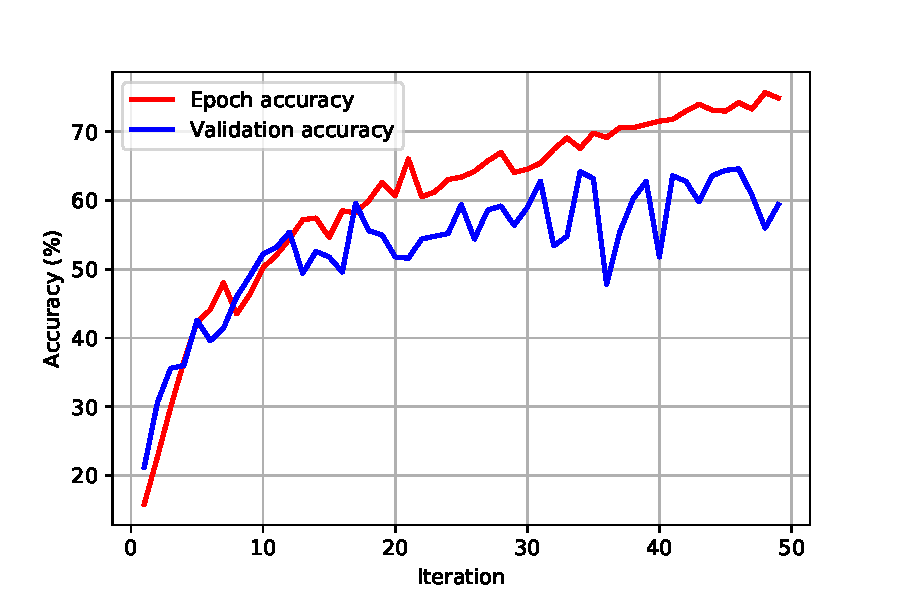
\includegraphics[width=6cm]{./results/baseline_pre_out_7_in_7_cifar10nore_5percent_acc.pdf}
	}
	\subfloat[][]
	{\hspace{-7mm}
		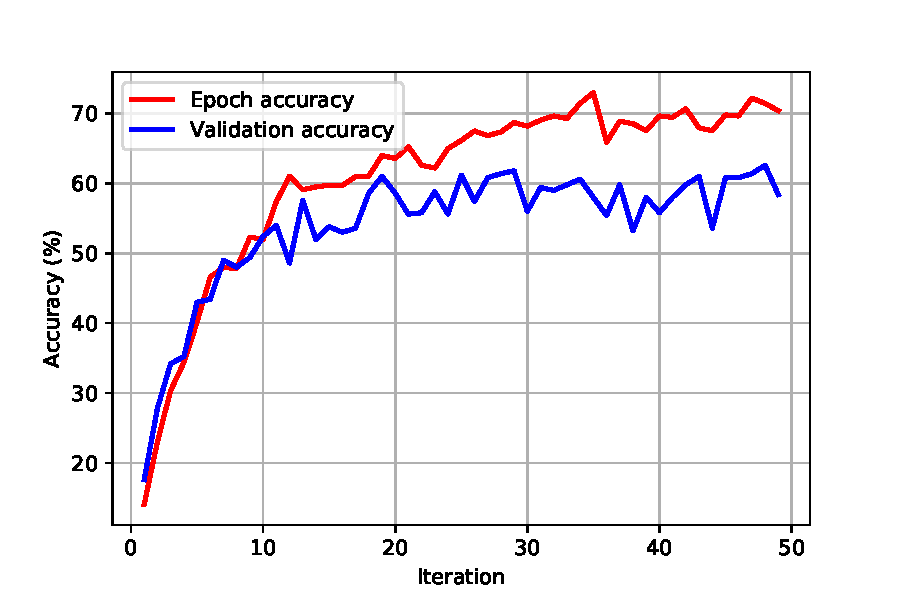
\includegraphics[width=6cm]{./results/pPruneWActNoNorm5_pre_out_7_in_7_cifar10nore_5percent_acc.pdf}
	}
	\subfloat[][]
	{\hspace{-7mm}
		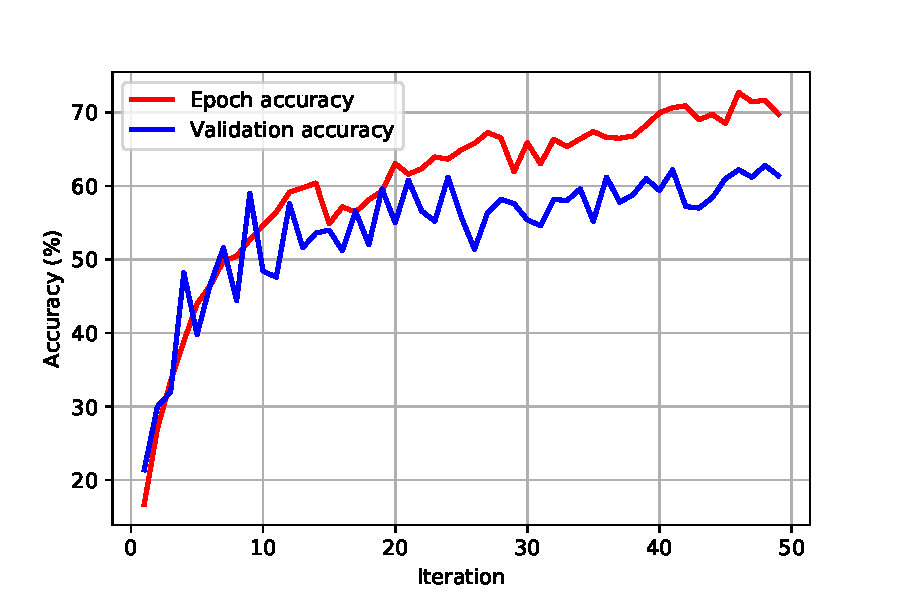
\includegraphics[width=6cm]{./results/pPruneWeightNoNorm5_pre_out_7_in_7_cifar10nore_5percent_acc.pdf}
	}\\[-5mm]
	\subfloat[][]
	{\hspace{-11mm}
		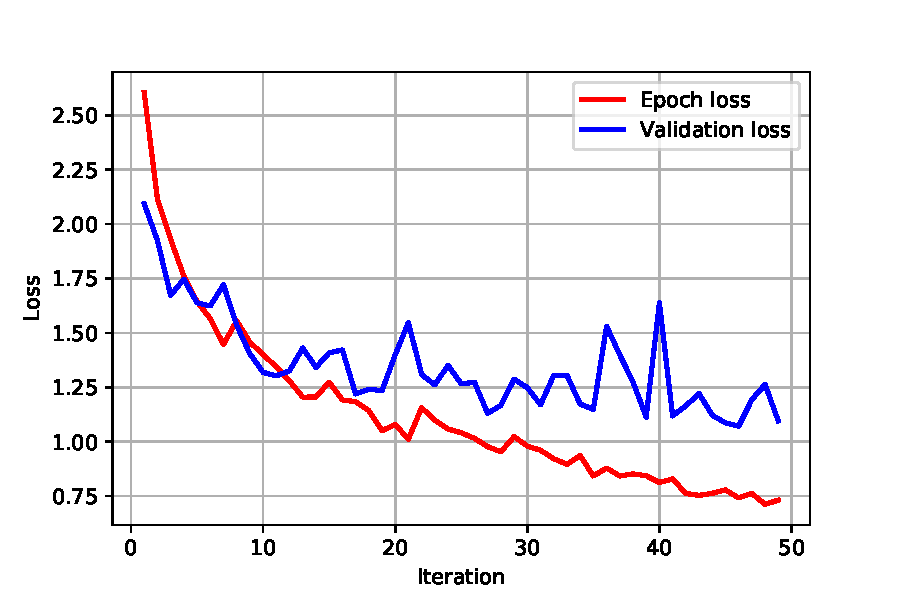
\includegraphics[width=6cm]{./results/baseline_pre_out_7_in_7_cifar10nore_5percent_loss.pdf}
	}
	\subfloat[][]
	{\hspace{-7mm}
		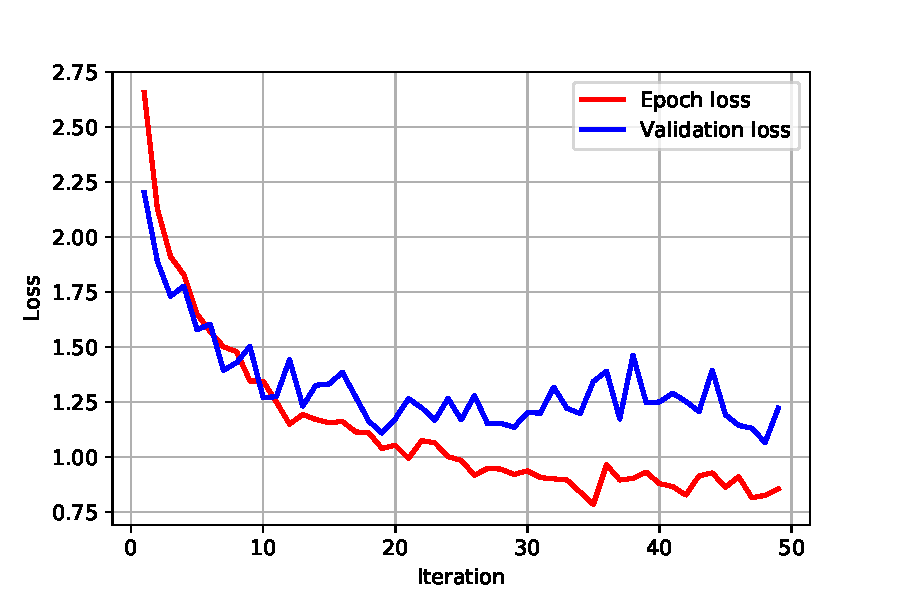
\includegraphics[width=6cm]{./results/pPruneWActNoNorm5_pre_out_7_in_7_cifar10nore_5percent_loss.pdf}
	}
	\subfloat[][]
	{\hspace{-7mm}
		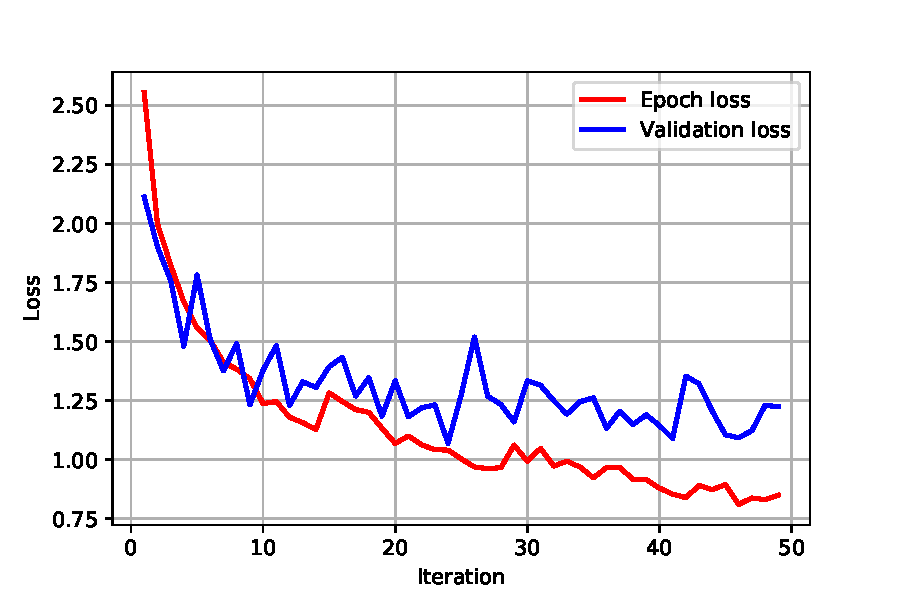
\includegraphics[width=6cm]{./results/pPruneWeightNoNorm5_pre_out_7_in_7_cifar10nore_5percent_loss.pdf}
	}
	\caption{\textbf{Filter pruning on a single dataset:} Accuracy and loss of pre-trained VGG16 during fine-tuning on $5$\% of CIFAR-10 data ($2000$ training images, $500$ validation images) for $50$ epochs. Top row: accuracy. Bottom row: loss. Left column: baseline model with no pruning. Middle column: activation-based pruning of $5$\% of all filters every $7$ epochs. Right column: weight-based pruning of $5$\% of all filters every $7$ epochs.}
	\label{pruneFiltersSingle}
\end{figure}


\subsection{Pruning with Multiple Datasets}
In this section we present and discuss the results pertaining to the combination of pruning algorithms with the idea of learning from multiple datasets for generalization.

\subsubsection{Intersection Pruning of Classifier Layers Based on a Threshold}

We next assessed the efficacy of iterative threshold pruning of classifier layers. We conducted the following experiments:
\begin{itemize}
	\item The first study involved training on a fixed subset of $800$ images from CIFAR-10 and training VGG-16 (pre-trained on ImageNet) for a total of $70$ epochs on that data subset. The weights with the $5$\% lowest absolute values in the first two classifier layers were set to zero, and the other weights continued training
.
	\item The second study involved drawing a different $800$-image subset from CIFAR-10 $10$ times and training a pre-trained VGG-16 for $7$ epochs on that dataset. The weights with the $5$\% lowest absolute values in the first two classifier layers were set to zero. Non-zero weights were then randomly re-initialized but the pruned weights remained zero for the remainer of training.

	\item Third, we assessed performance when drawing a different $800$-image dataset from one of $6$ datasets: CIFAR-10, CIFAR-100, MNIST, KMNIST, FashionMNIST and EMNIST. A total of $70$ epochs were run, sampling the datasets every $7$ epochs, while training a pre-trained VGG-16. The weights with the $5$\% lowest absolute values in the first two classifier layers were set to zero. The remaining weights continued training.

\end{itemize}

The main observations were the following:
\begin{itemize}
	\item Drawing dataset subsets from a single dataset and then applying threshold pruning led to comparable training and testing loss even when $>50$ of the weights are eliminated. The validation/training discrepancy was minimal, indicative of good generalization potential. As drawing multiple data subsets from a larger dataset is similar to training on a large dataset, these results suggest that periodic threshold pruning throughout training may be effective in a sufficiently large training set. The generalizability advantages could be seen most clearly when only the mask was retained across data subsets and weights were re-initialized. Validation accuracy remained near $50$\% while training accuracy dropped sharply. In line with the findings by \citet{prune_for_architecture}, these results suggest retained connections are more important to pruning than retained weights, and eliminating redundant weights can help reduce overfitting.
	\item In contrast, subsampling from different datasets led to sharp peaks in both the training and validation losses and drops in the accuracy throughout training. The datasets were likely too different for the classifier to learn meaningful weights or connections from each data subset using this approach.
	\item Together, these results demonstrate that intersection threshold pruning of classifier layers may be useful for improving generalization when applied to a large dataset, or closely-related data subsets.
\end{itemize}



\subsubsection{Meta-Pruning Classifier Layers}

As a proof of concept, we first assess the efficacy of L0 pruning in an $800$-sample data subset of CIFAR-10, trained for $20$ epochs using a pre-trained VGG16. Consistent with previous work, this effectively reduced the number of floating point operations while maintaining comparable accuracy to the baseline, as shown in \figref{f3}. However, we were unable to use this approach to train VGG16 from scratch, since the losses did not decrease, likely because the gradients were too unstable. 

Consistent with these findings, meta-pruning was ineffective for learning initial weights and L0 masks. Using $800$ image data subsets from CIFAR-10 for each of $20$ outer iterations, and training for $10$ epochs, did not reduce the final loss, the final number of floating point operations, or increase the final accuracy throughout training. The fluctuating trajectories suggest that learning was unstable, likely because the loss surface was very poorly conditioned. Using such small data-subsets likely gave a very weak gradient signal during the outer update and learning was unable to make meaningful progress. Larger data-subsets could increase the gradient signal, if more computational resources were available. Averaging the gradient signals or applying a momentum term could also help stabilize them.  Additionally, Reptile approximates the gradient updates using the difference between the final inner loop parameters and the outer loop parameters. Computing these more precisely, such as with MAML, may be necessary for meta-learning-based pruning architectures. 


\begin{figure}[!t]
	\centering
	\subfloat[][]
	{
		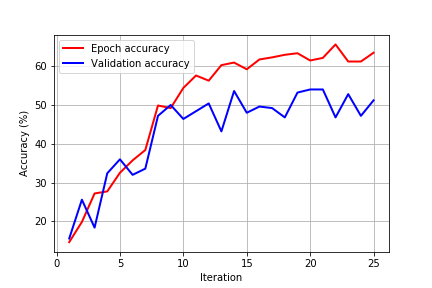
\includegraphics[width=6cm]{./Figures/Fig3/A_baseline_10_PT_accuracy.png}
	}
	\subfloat[][]
	{
		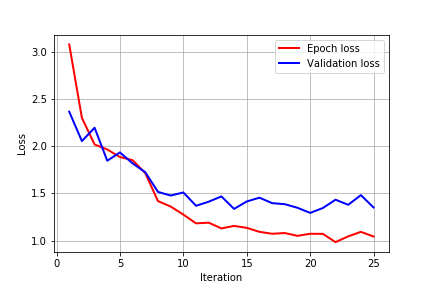
\includegraphics[width=6cm]{./Figures/Fig3/B_baseline_10_PT_loss.png}
	}\\
	\subfloat[][]
	{
		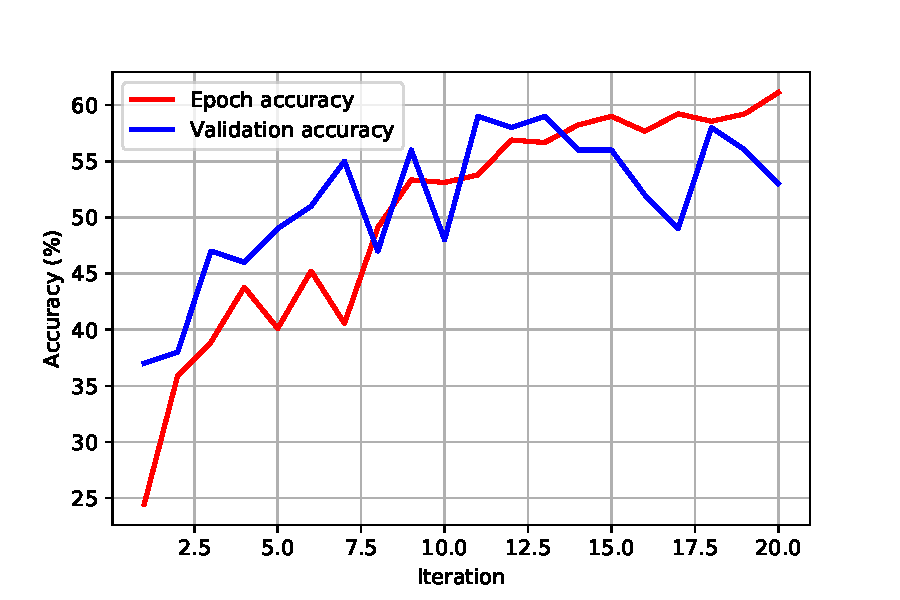
\includegraphics[width=6cm]{./Figures/Fig3/C_l0_weight_pruning_accuracy.pdf}
	}
	\subfloat[][]
	{
		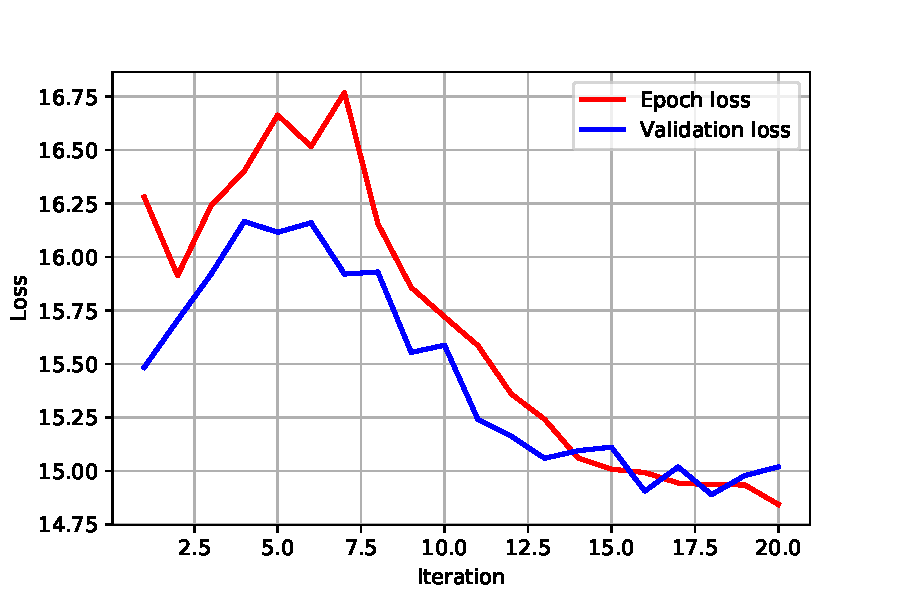
\includegraphics[width=6cm]{./Figures/Fig3/D_l0_weight_pruning_loss.pdf}
	}\\
	\subfloat[][]
	{
		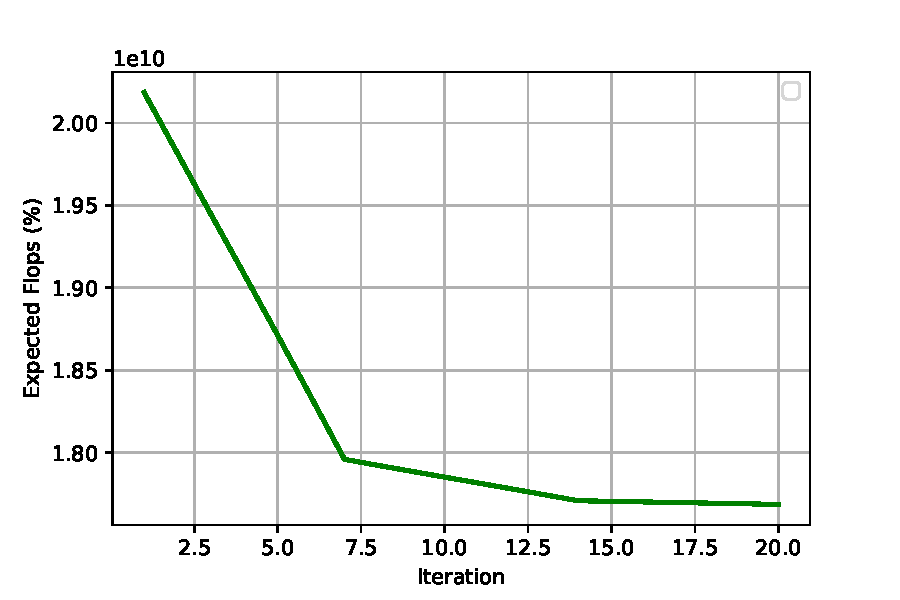
\includegraphics[width=6cm]{./Figures/Fig3/E_l0_weight_pruning_flop.pdf}
	}
	\subfloat[][]
	{
		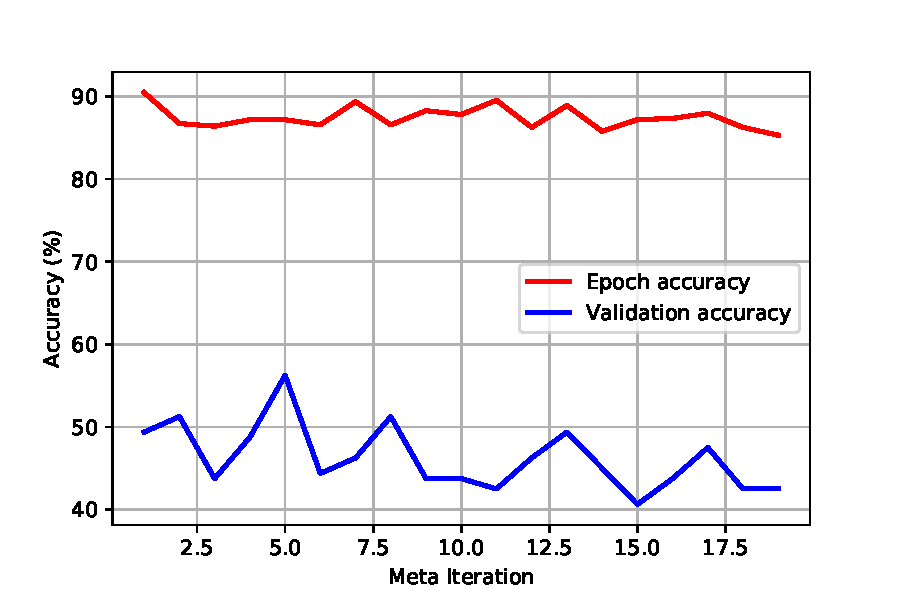
\includegraphics[width=6cm]{./Figures/Fig3/F_meta_pruning_02_800final_accuracy.pdf}
	}\\
	\subfloat[][]
	{
		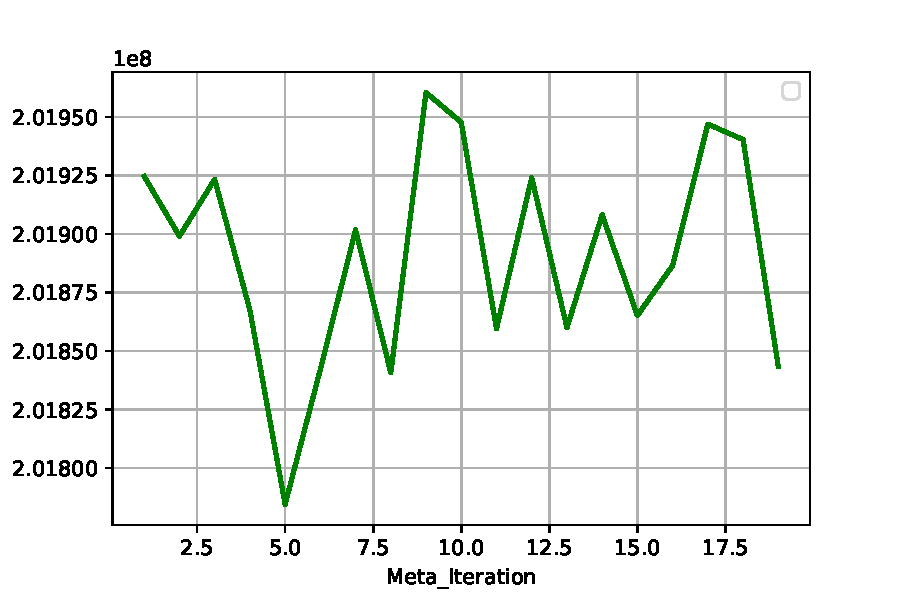
\includegraphics[width=6cm]{./Figures/Fig3/G_meta_pruning_02_800initial_flops.pdf}
	}
	\caption{A. Baseline accuracy on CIFAR-10 with pre-training. B. Baseline loss on CIFAR-10 with pre-training.  C. Accuracy on CIFAR-10 with pre-training and L0 regularization. D.  loss on CIFAR-10 with pre-training and L0 regularization. E.  expected number of floating point operations in the classifier for CIFAR-10 with pre-training and L0 regularization. F. Final meta-pruning accuracy with L0 regularisation on CIFAR-10. G. Final expected number of floating point operations in the classifier with L0 regularisation on CIFAR-10.}
	\label{f3}
\end{figure}

\subsubsection{Intersection Pruning of Convolution Filters}

The following two studies were conducted:
\begin{itemize}
	\item \textbf{Iterative subsampling from the same dataset}: In this study, training was performed on CIFAR-10, and $10$\% of the available data ($4000$ images) was resampled with replacement after every $N_i = 7$ epochs.
	This study is meant to be a toy example of the more realistic case when several similar datasets are available, along with the computational resources required to use larger numbers of training samples at each iteration.
	$5$\% of the network's convolutional filters were pruned every $N_i = 7$ epochs, based on the un-normalized 2-norms of the layers' weight matrices as well as their activations, as described above. This was compared to the baseline case of training the network in the same way, but without pruning. The results are shown in \figref{pruneFiltersIntersectionSubsample}.
	
	Unlike the results seen in \secref{PruneFilterRes}, the figures show that both filter pruning approaches studied here decrease training accuracy compared to the baseline model by approximately $10$\% on average. However, the validation accuracy is only $\sim 3$\% lower than that obtained with the baseline model, on average, but with $74$\% of the original network's filters. Although a larger proportion of the total CIFAR-10 dataset is represented during training, due to iterative subsampling, there is still a significant difference between training and validation accuracy in the baseline model (approximately $10$\%). However, the main result of this study is that in the pruned networks, performance on both training and validation data are very well balanced with respect to one another. This is a clear indicator that, as hypothesized, the pruned network shows better potential to generalize well, compared to the original network. The pruned network loss and accuracy are again much less stable over epochs than the original model, while the baseline model is much more stable. The fluctuations in the pruned model curves may be improved by pruning more gradually, for a larger number of epochs, and / or by using more sophisticated algorithms to pick which filters to prune.

	To further stress-test the impact of pruning the model more aggressively, we repeated the above study, subsampling $5$\% of available training data from CIFAR-10, for a total of $150$ epochs. $5$\% of the total network filters were pruned every $10$ epochs. The total number of filters was reduced by $50$\%, from $4224$ to $2117$. As a baseline, the same study was performed without pruning. The purpose was to see how far we can push the reduction in the number of filter, and the results are shown in \figref{pruneFiltersIntersectionSubsample2}. The jumps in accuracy correspond to resampling the dataset every $10$ epochs. The training accuracy plateaus around $68$\% in the pruned model, and is again closely tracked by the validation accuracy. The baseline model provides on average $5$\% percent better accuracy than the pruned model, but its validation accuracy is still within $\sim 1\text{--}3$\% of the pruned model, which again indicates better generalization. Additionally, it is clear that the baseline model starts to overfit, as evidenced by the increasing difference between training and validation accuracy. However, this is not true for the pruned model; its validation accuracy consistently remains nearly as good as the training accuracy, further indicating better generalization. Furthermore, it took the pruned model $6.75$ minutes to train over final set of $10$\% epochs, while the baseline model took approximately $14.5$ minutes per $10$ epochs. Thus, it is to be expected that the pruned model will be at least twice as fast as the original upon deployment, in addition to potentially improved generalizability.
	
	\item \textbf{Iterative sampling from multiple datasets}: In this study, training was performed by sampling $5$\% of available training data from six different datasets provided via \texttt{torchvision}.
	A different dataset was sampled every $N_i = 6$ epochs.
	A total of 120 epochs were run, so that every dataset was sampled twice.
	The six datasets used were CIFAR-10, CIFAR-100, MNIST, KMNIST, FashionMNIST and EMNIST.
	This study is meant to be a stress-test where the model is fine-tuned and pruned based on multiple datasets with images of very different categories. $5$\% of the network's convolutional filters were pruned every $N_i = 6$ epochs, based on the un-normalized 2-norms of the layers' weight matrices. This was compared to the baseline case of training the network in the same way, but without pruning. The results are shown in \figref{pruneFiltersIntersectionMultiple}.
	
	The sudden jumps in the figures indicate when a new dataset was sampled. The first six sets of peaks correspond to the first pass over each different dataset, while the last set of six peaks corresponds to the second pass over each dataset. Two major observations can be made from these results:
	
	\begin{enumerate}
		\item Overall, it is seen that in both the baseline and pruning cases, the accuracy improves during the second pass over the same dataset. Although this seems to be obviously expected, it is an important observation, for the following reason: between the first and the second time that the same dataset it encountered, the model trains on five other datasets in between (with possibly a completely different set of categories and image types). One may expect these intermediate epochs to hurt the model's performance on each previous dataset it was trained on. However, it seems that the model becomes relatively robust to be being trained on multiple different datasets; in other words, introducing it to a new dataset does not make it ``forget'' what was learned on previous datasets. This indicates that training on multiple datasets does indeed hold promise in making networks generalize well. However, an important point to remember is that each time a new dataset is encountered, the classifier layer weights will change significantly to learn the possible categories of that dataset. So at the end of training, the network will only perform well when tested on the last dataset encountered. To test on a different dataset, a very small amount of fine-tuning only the classifier is needed. However, our claim is that fine-tuning the entire network on multiple datasets should mean that minimal fine-tuning of the classifier should be required when switching among datasets.
		\item Both the pruned and original baseline models perform equally well in general; in fact it requires careful observation of the curves to see where they differ in their performance. However, the total number of convolution filters in the pruned model, after 120 epochs, was reduced from $4224$ to $2449$, which is a $42$\% reduction in the size of the network, not counting the classifier layer.
	\end{enumerate}
	In summary, these results indicate that pruning a network to $58$\% of its original size can be achieved while maintaining its performance, and also maintaining or possibly improving its ability to generalize, compared to the baseline model.
	
\end{itemize}

\begin{figure}[!t]
	\centering
	\subfloat[][]
	{\hspace{-11mm}
		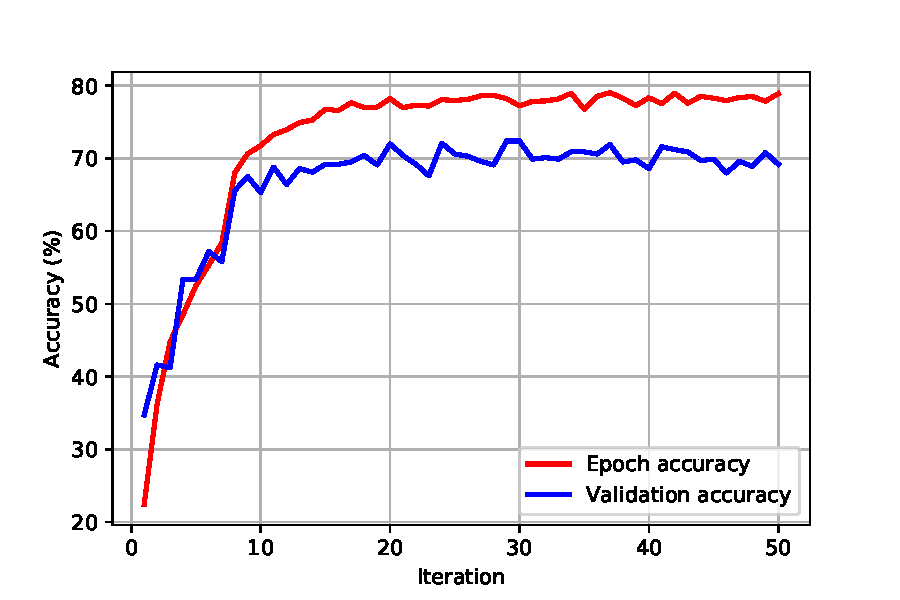
\includegraphics[width=6cm]{./results/baseline_pre_out_1_in_50_cifar10_10percent_acc.pdf}
	}
	\subfloat[][]
	{\hspace{-7mm}
		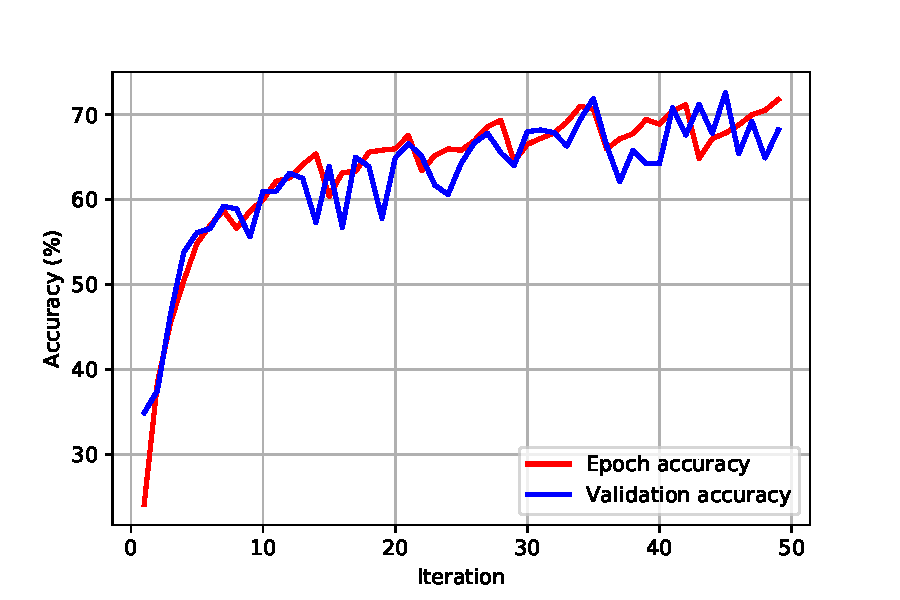
\includegraphics[width=6cm]{./results/pPruneActNoNorm5_pre_out_7_in_7_cifar10_10percent_acc.pdf}
	}
	\subfloat[][]
	{\hspace{-7mm}
		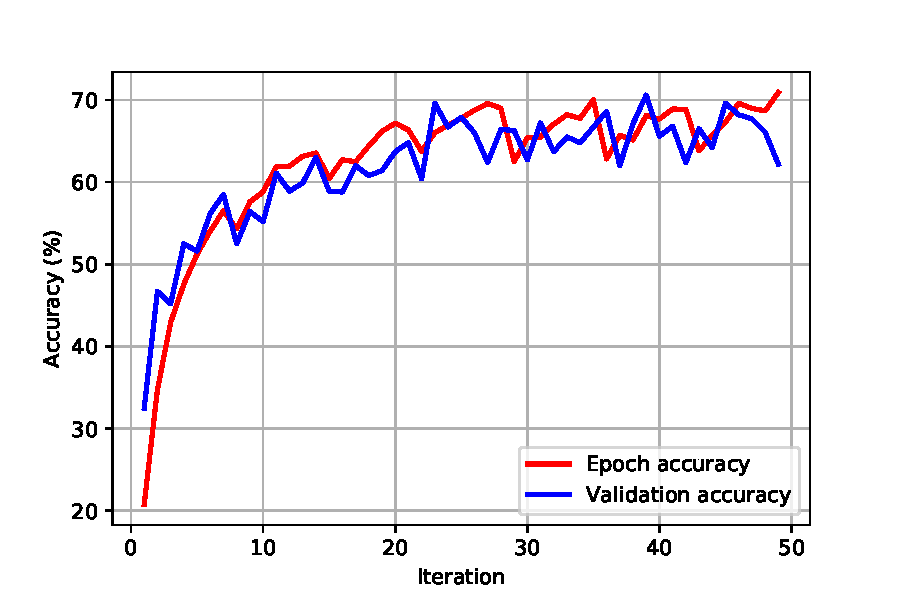
\includegraphics[width=6cm]{./results/pPruneWeightNoNorm5_pre_out_7_in_7_cifar10_10percent_acc.pdf}
	}\\[-5mm]
	\subfloat[][]
	{\hspace{-11mm}
		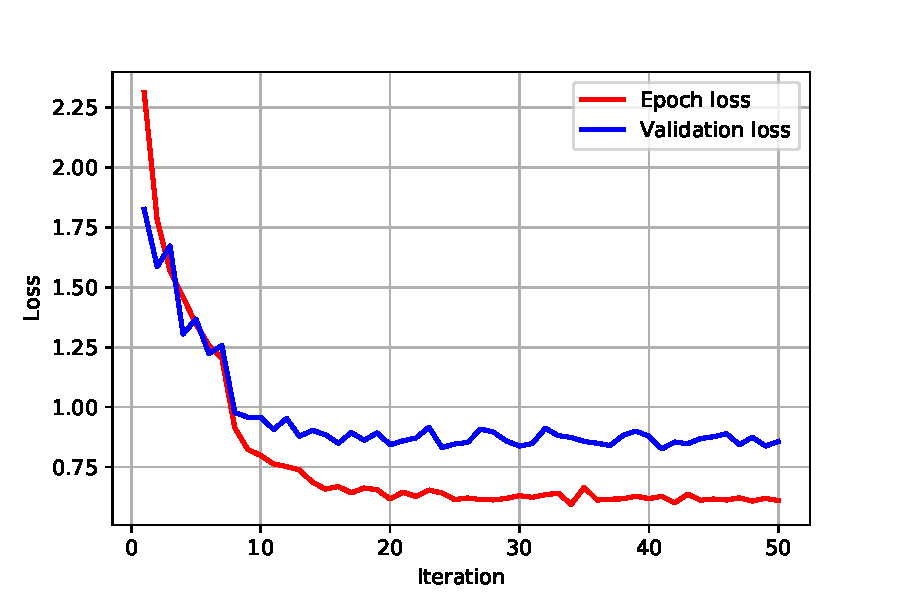
\includegraphics[width=6cm]{./results/baseline_pre_out_1_in_50_cifar10_10percent_loss.pdf}
	}
	\subfloat[][]
	{\hspace{-7mm}
		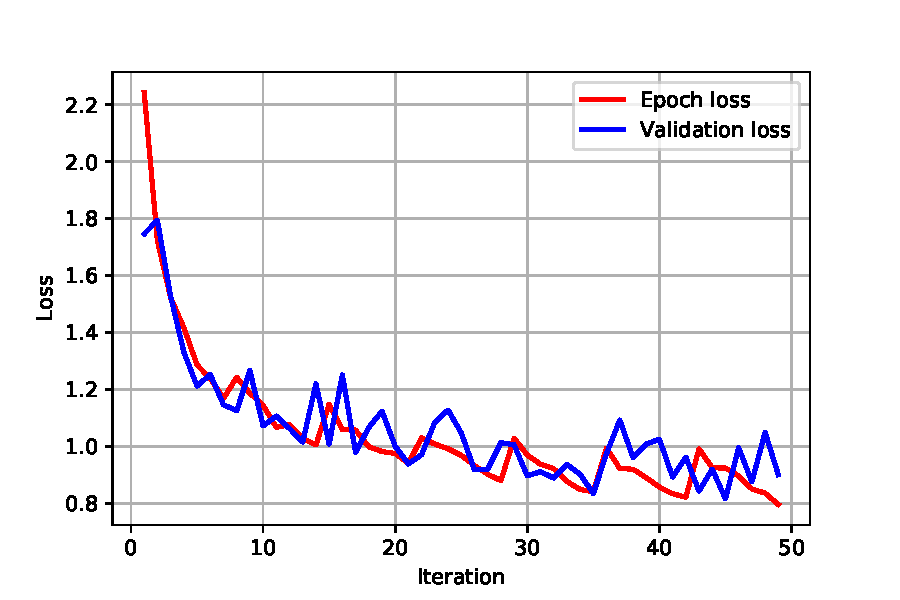
\includegraphics[width=6cm]{./results/pPruneActNoNorm5_pre_out_7_in_7_cifar10_10percent_loss.pdf}
	}
	\subfloat[][]
	{\hspace{-7mm}
		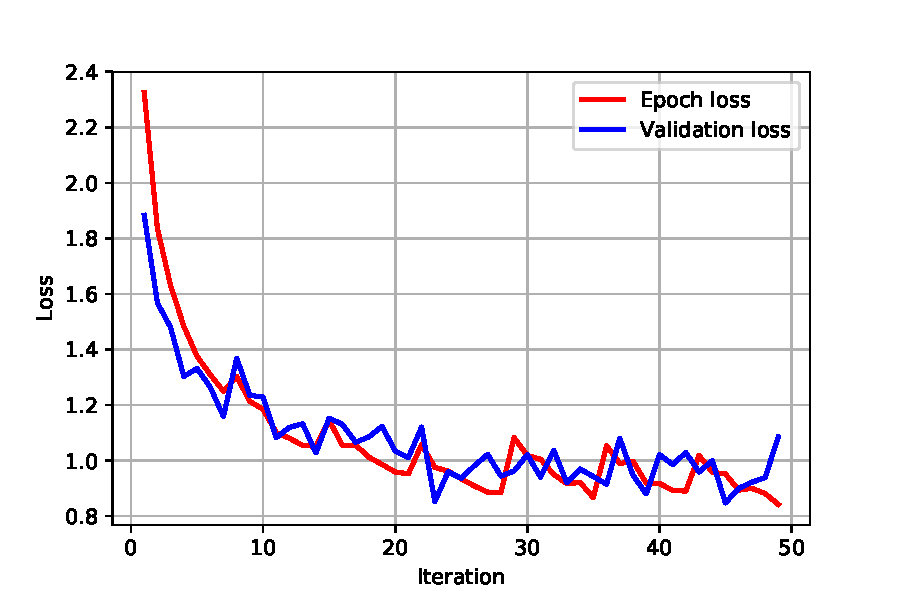
\includegraphics[width=6cm]{./results/pPruneWeightNoNorm5_pre_out_7_in_7_cifar10_10percent_loss.pdf}
	}
	\caption{\textbf{Iterative subsampling from CIFAR-10:} Accuracy and loss of pre-trained VGG16 during fine-tuning. Top row: accuracy. Bottom row: loss. Left column: baseline model with no pruning. Middle column: activation-based pruning of $5$\% of all filters every $7$ epochs. Right column: weight-based pruning of $5$\% of all filters every $7$ epochs.}
	\label{pruneFiltersIntersectionSubsample}
\end{figure}

\begin{figure}[!t]
	\centering
	\subfloat[][]
	{
		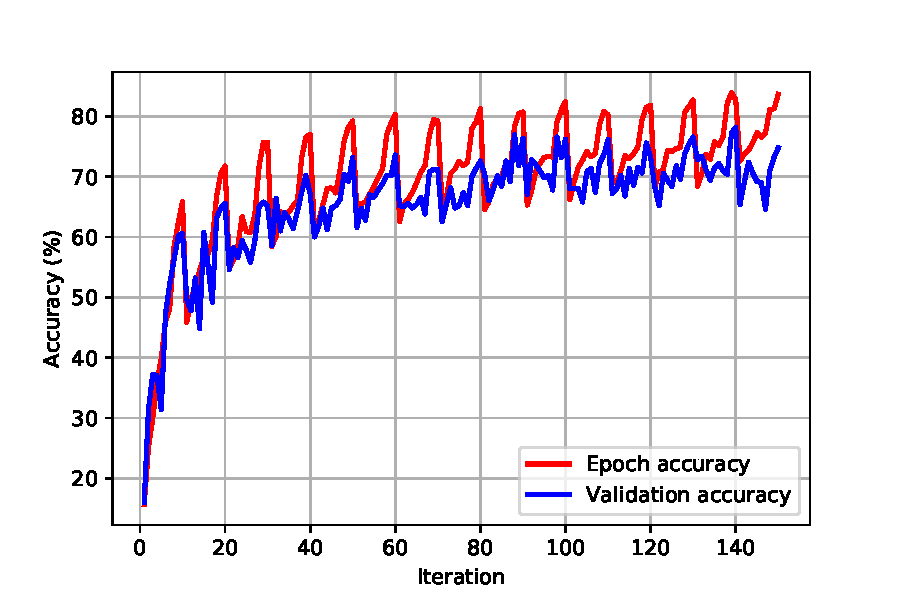
\includegraphics[width=7cm]{./results/baseline_pre_out_15_in_10_cifar10_5percent_acc.pdf}
	}
	\subfloat[][]
	{
		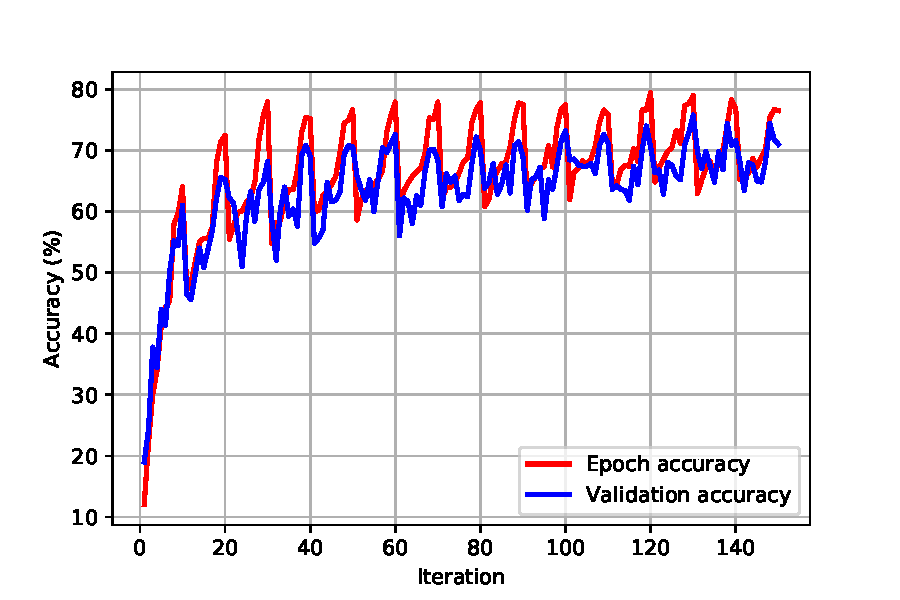
\includegraphics[width=7cm]{./results/pPruneWeightNoNorm5_pre_out_15_in_10_cifar10_5percent_acc.pdf}
	}\\[-5mm]
	\subfloat[][]
	{
		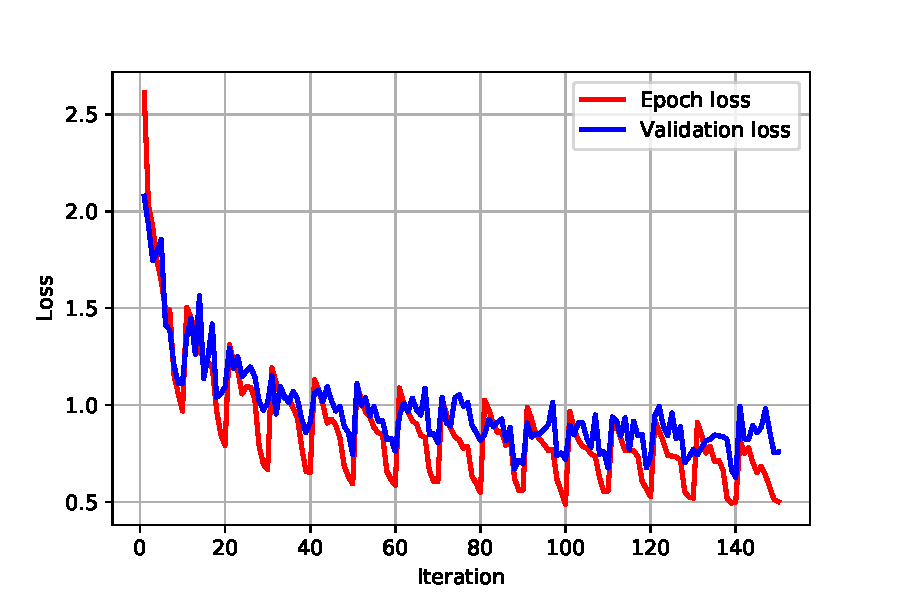
\includegraphics[width=7cm]{./results/baseline_pre_out_15_in_10_cifar10_5percent_loss.pdf}
	}
	\subfloat[][]
	{
		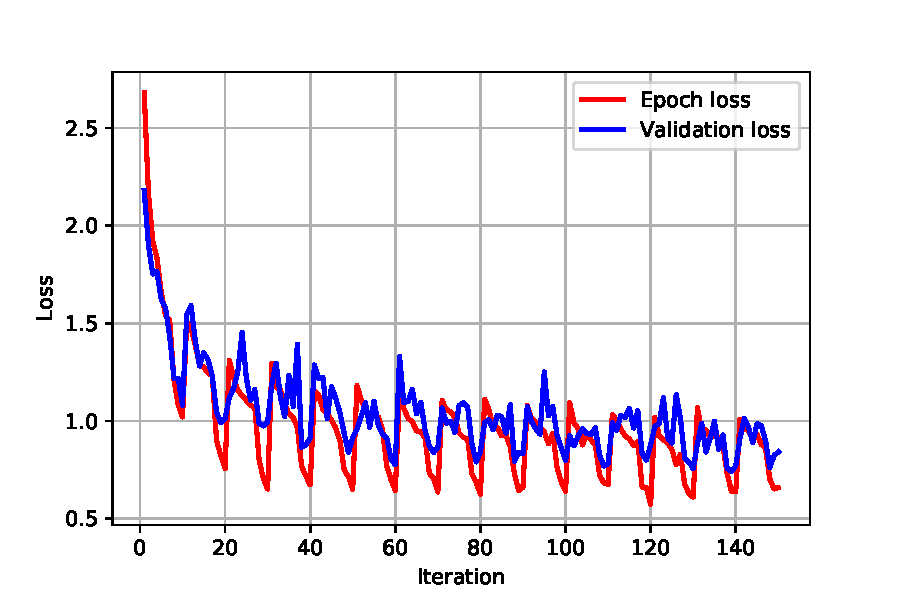
\includegraphics[width=7cm]{./results/pPruneWeightNoNorm5_pre_out_15_in_10_cifar10_5percent_loss.pdf}
	}
	\caption{\textbf{Iterative subsampling from CIFAR-10:} Accuracy and loss of pre-trained VGG16 during fine-tuning. Top row: accuracy. Bottom row: loss. Left column: baseline model with no pruning. Right column: weight-based pruning of $5$\% of all filters every $10$ epochs.}
	\label{pruneFiltersIntersectionSubsample2}
\end{figure}

\begin{figure}[!t]
	\centering
	\subfloat[][]
	{
		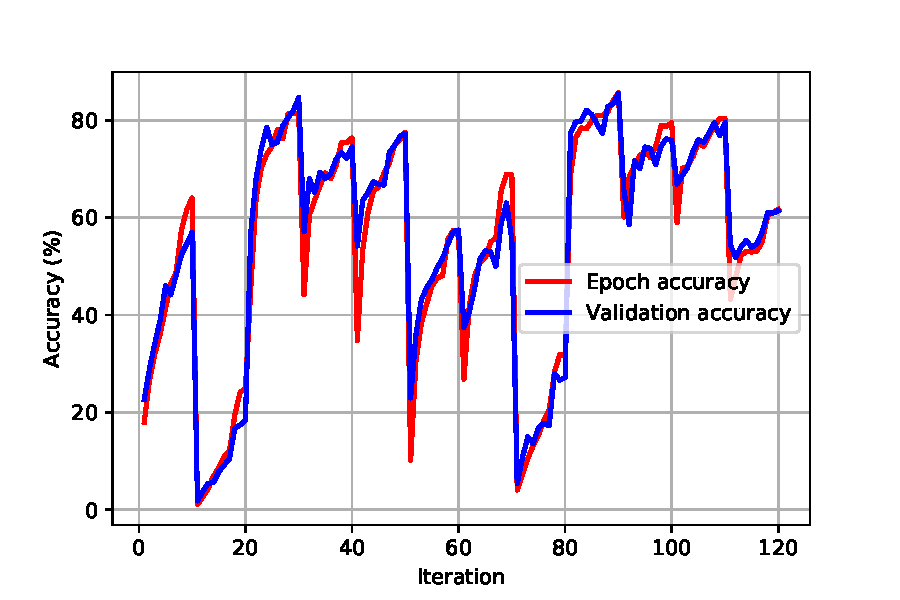
\includegraphics[width=7cm]{./results/baseline_pre_out_12_in_10_multiple_5percent_acc.pdf}
	}
	\subfloat[][]
	{
		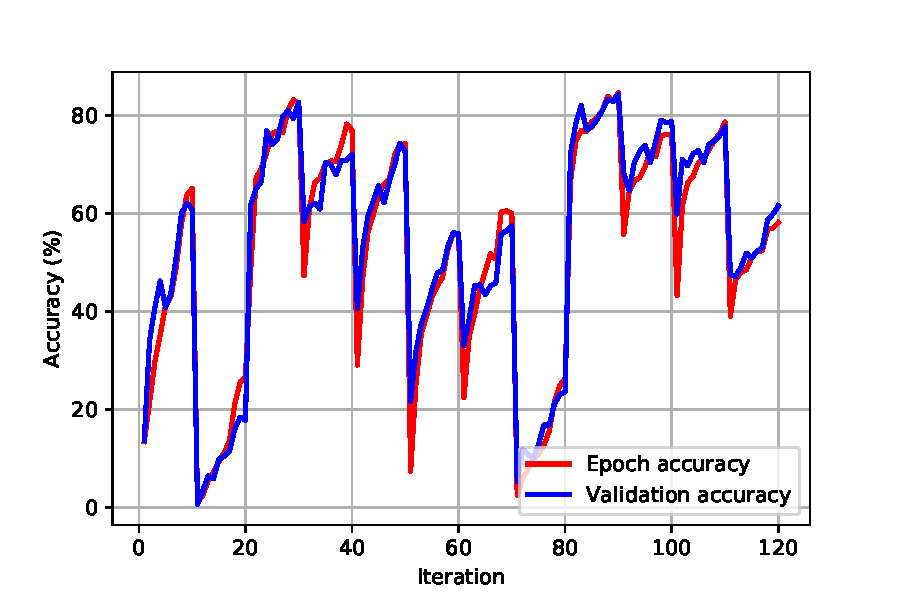
\includegraphics[width=7cm]{./results/pPruneWeightNorm5_pre_out_12_in_10_multiple_5percent_acc.pdf}
	}\\[-5mm]
	\subfloat[][]
	{
		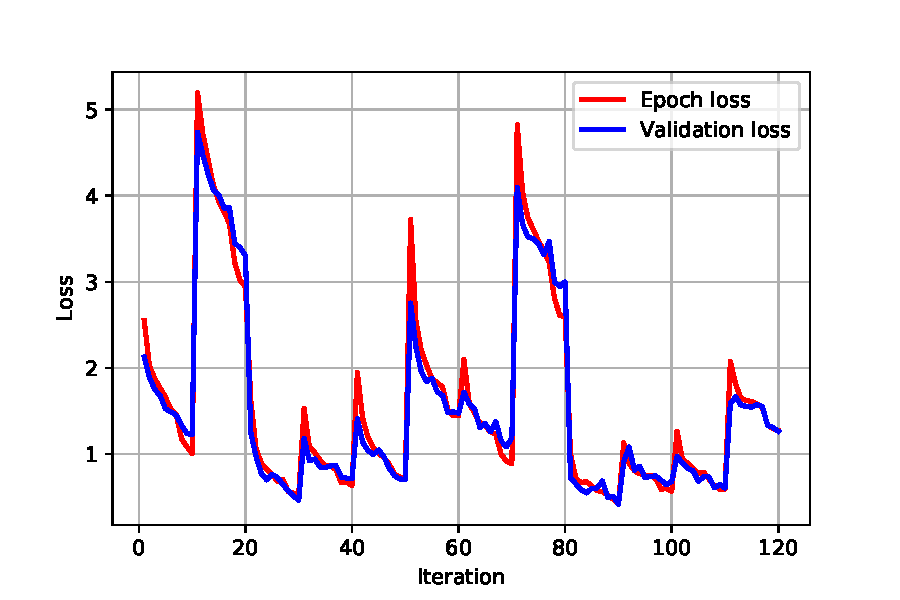
\includegraphics[width=7cm]{./results/baseline_pre_out_12_in_10_multiple_5percent_loss.pdf}
	}
	\subfloat[][]
	{
		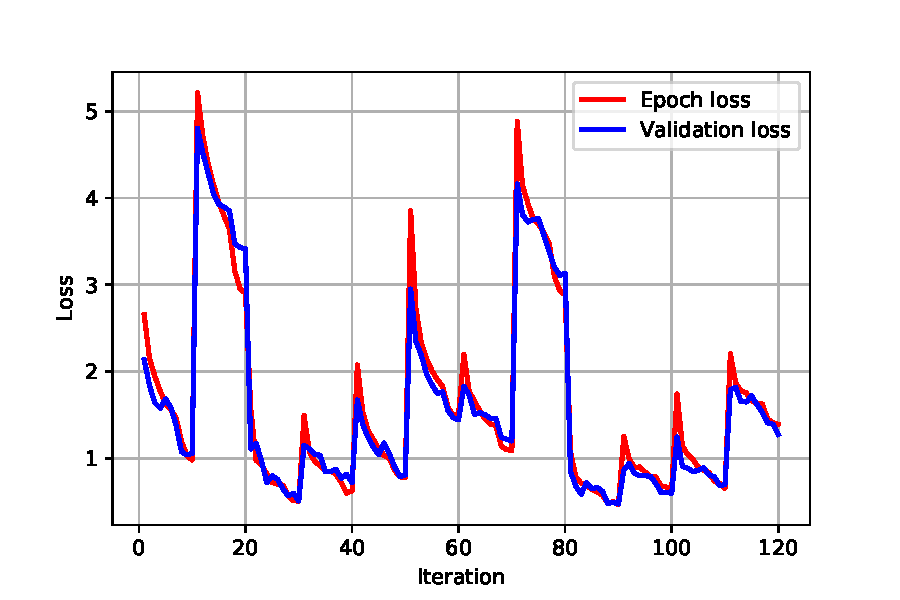
\includegraphics[width=7cm]{./results/pPruneWeightNorm5_pre_out_12_in_10_multiple_5percent_loss.pdf}
	}
	\caption{\textbf{Iterative sampling from multiple datasets:} Accuracy and loss of pre-trained VGG16 during fine-tuning. Top row: accuracy. Bottom row: loss. Left column: baseline model with no pruning. Right column: weight-based pruning of $5$\% of all filters every $6$ epochs.}
	\label{pruneFiltersIntersectionMultiple}
\end{figure}


\section{Limitations}

Some of the major limitations of the proposed methodologies are:
\begin{itemize}
	\item Relatively simple metrics are used to determine what to prune, and the gradients of the loss with respect to network parameters have not been taken into account, unlike existing works in literature.
	\item The process of repeatedly sampling from different datasets would work much better if there was a larger overlap between their image categories, and were more closely related. Since we only used datasets easily available via \texttt{torchvision}, the choices were limited. However, even if the datasets were more closely related, they could also just be combined into one large dataset, so the benefit of resampling seems quite limited.
	\item In threshold masking, one limitation is that weights that are masked once can not come back. We attempted to alleviate this via meta-pruning, but it did not seem to work very well.
	\item We have not thoroughly quantified network performance with pruning in terms of memory and power consumption.
	\item The only GPUs we had access to were through Google Colaboratory, which limited the amount of training data we could use within the time constraints.
	\item We have only explored VGG16 - it would be interesting to study pruning on other networks, particularly those that rely on dropout.
\end{itemize}

\section{Conclusions}

In this work, we have surveyed simple techniques to prune large neural networks, using VGG16 as our test model. Due to the potential for pruning to improve network generalization, we have also attempted to combine pruning with the concept of meta-learning in two ways: one is by iteratively sampling from different but related datasets (``intersection pruning''), and the other is by learning mask matrices which are applied to classifier layers (``meta-pruning''). We found that pruning does indeed allow a significant reduction in network size with a corresponding test-time speed-up. However, in the case of intersection pruning of filter weights, this comes with up to $10$\% reduction in training accuracy, but without a significant reduction in validation accuracy. This indicates potentially better generalization properties of the pruned model. It was also observed that when sampling from multiple datasets, pruning filters has a very minor effect on both training and validation accuracy.

\section{List of Contributions}

The work discussed in this paper is not in any way related to either authors' research or other activities, and was done purely for the purpose of submission as a project for CSC2516 at the University of Toronto. Specific contributions of each author are listed in \tabref{contr}.

\begin{table}[!h]
	\centering
	\caption{Contributions of each author.}
	\begin{tabular}{lll}
		\toprule
		& Adriana & Shashwat \\
		\midrule
		Code & Formulated and coded threshold-based & Formulated  and coded activation- and weight- \\
		& masking of weights in the classifier & based pruning of convolution layer filters \\[2mm]
		& Discovered and implemented L0-based & Extended Adriana's implementation \\
		& masking of classifier layers & of L0-based masking for convolution layers \\[2mm]
		& Discovered and implemented REPTILE & Wrote basic data-loading and visualization \\
		& meta-learning to learn classifier masks & interfaces for the various studies \\[2mm]
		Writeup & Wrote all sections pertaining to & Wrote all sections pertaining to \\
		& classifier masking & filter pruning\\[2mm]
		& Wrote all sections pertaining to & Wrote the introduction \\
		& REPTILE meta-learning & \\[2mm]
		& Wrote the related work section & Typesetting in \LaTeX \\[2mm]
		& Editing & Editing \\[2mm]
		Overall & $\sim 60$\% of total work done in this project & $\sim 40$\% of total work done in this project \\
		\bottomrule
	\end{tabular}
	\label{contr}
\end{table}

\subsubsection*{Acknowledgments}

We would like to thank the instructors (Roger Grosse and Jimmy Ba) and TAs of CSC2516 for providing a valuable learning experience through this course.

\bibliographystyle{apalike} % IEEEtran is only available via some tex installations. Can change to any other, e.g. "plain".
\bibliography{references}

%\section*{References}
%
%References follow the acknowledgments. Use unnumbered first-level heading for
%the references. Any choice of citation style is acceptable as long as you are
%consistent. It is permissible to reduce the font size to \verb+small+ (9 point)
%when listing the references. {\bf Remember that you can use more than eight
%  pages as long as the additional pages contain \emph{only} cited references.}
%\medskip
%
%\small
%
%[1] Alexander, J.A.\ \& Mozer, M.C.\ (1995) Template-based algorithms for
%connectionist rule extraction. In G.\ Tesauro, D.S.\ Touretzky and T.K.\ Leen
%(eds.), {\it Advances in Neural Information Processing Systems 7},
%pp.\ 609--616. Cambridge, MA: MIT Press.
%
%[2] Bower, J.M.\ \& Beeman, D.\ (1995) {\it The Book of GENESIS: Exploring
%  Realistic Neural Models with the GEneral NEural SImulation System.}  New York:
%TELOS/Springer--Verlag.
%
%[3] Hasselmo, M.E., Schnell, E.\ \& Barkai, E.\ (1995) Dynamics of learning and
%recall at excitatory recurrent synapses and cholinergic modulation in rat
%hippocampal region CA3. {\it Journal of Neuroscience} {\bf 15}(7):5249-5262.

\end{document}
